%----------------------------------------------------------------------------------------
%	THESIS
%   Protection mechanisms for electronic books
%
%----------------------------------------------------------------------------------------
% License:
% This work is licensed under the Creative Commons Attribution-NonCommercial-ShareAlike 4.0 International License. To view a copy of this license, visit http://creativecommons.org/licenses/by-nc-sa/4.0/.
%
% Author:
% Patrick Ausderau
%
% Date: July 2012 - May 2014
%
% Note:
% This LaTeX file served as a basis for and benefit from the "Metropolia Thesis LaTeX Template" (CC-BY) with the help of Panu Lepp�niemi and Patrik Luoto. The template can be found at https://github.com/panunu/metropolia-thesis-latex. Happy thesis writting!

\author{Patrick Ausderau}
\title{Protection mechanisms for electronic books}

\date{\today}
\def\metropoliadegree {Master of Engineering}
%Master Degree Programme in Information Technology
\def\metropoliadegreeprogramme {Information Technology}
\def\metropoliaspecialisation {Mobile Programming}
\def\metropoliainstructors {
Olli Alm, Project Manager\newline
Harri Airaksinen, Head of Degree Programme
}
\def\metropoliakeywords {Electronic book (e-book), EPUB, PDF, Digital Right Management (DRM), Social DRM, Watermark, Copyright, DRM-free}

%----------------------------------------------------------------------------------------
%	GLOBAL STYLES
%----------------------------------------------------------------------------------------

\documentclass[11pt,a4paper,oneside]{memoir}
\usepackage[latin1]{inputenc}
\usepackage{amsmath}
\usepackage{amsfonts}
\usepackage{amssymb}
\usepackage{fontspec}
\usepackage{tocloft}
\usepackage{lipsum}
\usepackage{titlesec}
\usepackage[hyphens]{url}
%\usepackage{mathtools}
\usepackage{wallpaper}
%\usepackage{eso-pic}
\usepackage{datetime}
\usepackage{url}
%\usepackage[amssymb]{SIunits}
%\renewcommand{\dateseparator}{.}
%condition for adding or not space in TOC
\usepackage{etoolbox}
%for compact list
\usepackage{enumitem}
%for block comment
\usepackage{verbatim}
%for "easier" references
\usepackage{varioref}
%forcing single line spacing in bibliography
\DisemulatePackage{setspace}
\usepackage{setspace}
%including figure (image)
\usepackage{graphicx}
%change the numbering for figure
\usepackage{chngcntr}
%strike trough
\usepackage{ulem}
%euro symbol
\usepackage{eurosym}
%try to count
\usepackage{totcount}
%insert source code
\usepackage{listings}
\usepackage{caption}
\usepackage{color}
%force the width of a table instead of column
\usepackage{tabu}


%NORMAL TEXT
%all text, title, etc. in same arial font
\setmainfont{Arial}
%\setmainfont{DejaVu Sans}
%line space
\linespread{1.5}
%\doublespacing
%margin
\usepackage[top=2.5cm, bottom=3cm, left=4cm, right=2cm, nofoot]{geometry}
\setlength{\parindent}{0pt}%first line of paragraph not indented
\setlength{\parskip}{16.5pt}%one empty line to separate paragraph
%list with small line space separation
\tightlists

%IMAGE - FIGURE
%the figures are in "img" folder.
\graphicspath{{img/}}
%figure number without chapter (1.1, 1.2, 2.1) to (1, 2, 3)
\counterwithout{figure}{chapter}
%border around images
\setlength\fboxsep{0pt}
\setlength\fboxrule{0.5pt}
%caption font size
\captionnamefont{\small}
\captiontitlefont{\small}
%space after figure caption (and other float elements)
\setlength{\belowcaptionskip}{-7pt}

%TABLE
\counterwithout{table}{chapter}
%space before table caption (and other float elements)
\setlength{\abovecaptionskip}{7pt}

%SOURCE CODE
\definecolor{darkgray}{rgb}{.4,.4,.4}
\definecolor{purple}{rgb}{0.65, 0.12, 0.82}
\lstdefinelanguage{JavaScript}{
  keywords={break, case, catch, continue, debugger, default, delete, do, else, false, finally, for, function, if, in, instanceof, new, null, return, switch, this, throw, true, try, typeof, var, void, while, with},
  morecomment=[l]{//},
  morecomment=[s]{/*}{*/},
  morestring=[b]',
  morestring=[b]",
  ndkeywords={class, export, boolean, throw, implements, import, this},
  ndkeywordstyle=\color{darkgray}\bfseries,
  sensitive=true
}
\lstset{
extendedchars=true,
captionpos=b,
caption=\footnotesize,
basicstyle=\singlespacing\ttfamily,%\small\fontfamily{"Courier"}\selectfont,
keywordstyle=\color{blue}\bfseries,
commentstyle=\color{purple}\itshape,
identifierstyle=\color{black},
stringstyle=\color{red},
showstringspaces=false,
showspaces=false,
numbers=left,
numberstyle=\footnotesize,
numbersep=9pt,
breaklines=true,
tabsize=2,
showtabs=false,
xleftmargin=1cm
}
%\counterwithout{lstlisting}{chapter}
%moved after begin document, otherwise does not compile

%TOC
%remove dots.
\renewcommand*{\cftdotsep}{\cftnodots}
%chapter title and page number not in bold.
\renewcommand{\cftchapterfont}{}
\renewcommand{\cftchapterpagefont}{}
%sub section in toc
\setcounter{tocdepth}{2}
%subsection numbered
\setcounter{secnumdepth}{2}
%\cfttoctitlefont{\normalfont\MakeUppercase}
\renewcommand{\tocheadstart}{\vspace*{-15pt}}
\renewcommand{\printtoctitle}[1]{\fontsize{13pt}{13pt}\bfseries #1}
\renewcommand{\aftertoctitle}{\vspace*{-22pt}\afterchaptertitle}
%spacing afer a chapter in toc
\preto\section{%
  \ifnum\value{section}=0\addtocontents{toc}{\vskip11pt}\fi
}
%spacing afer a section in toc
\renewcommand{\cftsectionaftersnumb}{\vspace*{-3pt}}
%spacing afer a subsection in toc
\renewcommand{\cftsubsectionaftersnumb}{\vspace*{-1pt}}
%appendix
\renewcommand*{\cftappendixname}{Appendix\space}

%TITLES
%chapter title
\titleformat{\chapter}
{\fontsize{13pt}{13pt}\bfseries\linespread{1}}
{\thechapter}{.5cm}{}
\titlespacing*{\chapter}{0pt}{.32cm}{9pt}
\titleformat{\section}
{\fontsize{12pt}{12pt}\linespread{1}}
{\thesection}{.5cm}{}
\titlespacing*{\section}{0pt}{14pt}{6pt}
\titleformat{\subsection}
{\fontsize{12pt}{12pt}\linespread{1}}
{\thesubsection}{.5cm}{}
\titlespacing*{\subsection}{0pt}{14pt}{6pt}

%QUOTE
\renewenvironment{quote}
    {\list{}{\rightmargin=0pt\leftmargin=1cm\topsep=-10pt}%
    \item\relax\fontsize{10pt}{10pt}\singlespacing}
    {\endlist}

%BIBLIOGRAPHY
%bibliography title to be "refercences"
\renewcommand\bibname{References}
\makeatletter % Reference list option change
\renewcommand\@biblabel[1]{#1\hspace{1cm}} % from [1] to 1 with 1cm gap
\makeatother %
%\makeatletter %
%\renewcommand\@bibitem{\linespread{0.5}} %
%\makeatother %
%\setlength{\bibitem}{16.5pt}
\setlength{\bibitemsep}{11pt}

%count the appendices (since the counter is reset after \appendix)
\regtotcounter{chapter}

%TITLE PAGE
\newcommand\BackgroundPic{%
\put(0,0){%
\parbox[b][\paperheight]{\paperwidth}{%
\vfill
\centering
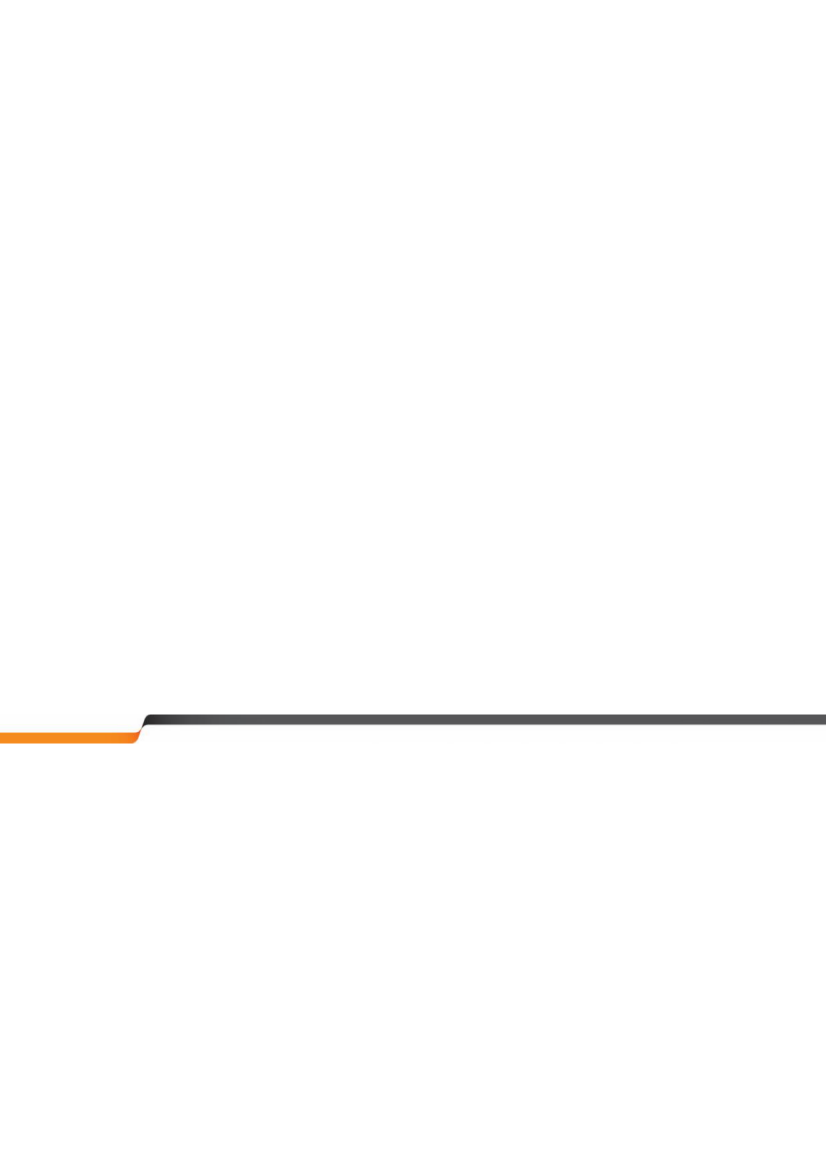
\includegraphics[width=\paperwidth,height=\paperheight,%
keepaspectratio]{viiva}%
\vfill
}}}

\makeatletter
\renewcommand{\maketitle}{
\thispagestyle{empty}
\ThisCenterWallPaper{1}{viiva}
%
\vspace*{9.5cm}
\tn{\LARGE \@author\\[0.75cm]\Huge \@title}\\[3.5cm]

\parbox{.7\linewidth}{\normalsize 
Helsinki Metropolia University of Applied Sciences\\[2pt]
\metropoliadegree \\[2pt]
\metropoliadegreeprogramme \\[2pt]
Thesis\\[2pt]
\ddmmyyyydate\today}%to be checked date format? 

\ThisLRCornerWallPaper{1}{metropolia}
%
\clearpage
}
\makeatother

\makepagestyle{abstract}
\makeevenhead{abstract}{}{}{Abstract}
\makeoddhead{abstract}{}{}{Abstract}



%==================== CONTENT ====================
\begin{document}
\counterwithout{lstlisting}{chapter}

\newcommand\tn[1]{\textnormal{#1}}
\newcommand\reaction[1]{\begin{equation}\ce{#1}\end{equation}}

%page number always on the top right. And clear the "chapter/section" head.
\pagestyle{myheadings}
\markright{}
%clear chapter "title" foot page.
\makeevenfoot{plain}{}{}{}
\makeoddfoot{plain}{}{}{}

%----------------------------------------------------------------------------------------
%	TITLE PAGE
%----------------------------------------------------------------------------------------

\maketitle
\newpage

%----------------------------------------------------------------------------------------
%	ABSTRACT
%----------------------------------------------------------------------------------------

\pagestyle{abstract}
\ThisLRCornerWallPaper{1}{footer}

\begin{tabular}{ | p{4,7cm} | p{10,3cm} |}
  \hline
  Author(s) \newline
  Title \newline\newline 
  Number of Pages \newline
  Date
  & 
  \makeatletter
  \@author \newline
  \@title \newline\newline
  \pageref{LastPage} pages + \total{chapter} appendices \newline %! if no appendices, risk to count total of chapter :D
  \@date
  \makeatother
  \\ \hline
  Degree & \metropoliadegree
  \\ \hline
  Degree Programme & \metropoliadegreeprogramme
  \\ \hline
  Specialisation option & \metropoliaspecialisation
  \\ \hline
  Instructor(s) & \metropoliainstructors
  \\ \hline
  \multicolumn{2}{|p{15cm}|}{\begin{singlespacing}\vspace{-22pt}
  The research for a new Digital Right Management (DRM) infrastructure for electronic books (e-book) is a task of the eReading work-package from the Next Media project, which goal is to to propose a protection system that could help limiting copyright infringement while allowing fair use of e-books.\newline
  
  This thesis reviews the existing technologies, like DRM, Watermark and Social DRM. It studies the upcoming Lightweight Content Protection standard (for EPUB). Apart from the technical aspect, the legal, educational and financial lewis to reduce copyright infringement are studied. Web crawler and its implication into finding infringing material on the internet is addition to this work. \newline
  
  The main outputs of this thesis are a deliverable (number 1.3.1.4) for the Next Media project, presentations, seminars and conferences to the Finnish National Library, Next Media project, Finnish Book Publishers Association and Finnish author unions and the participation to the redaction of the DRM recommendations for the Finnish Book Publishers Association members. \newline

  This thesis recommends not to use DRM to protect e-books but to use either a lighter protection mechanism such as Watermark and Social DRM combination or to be DRM-free. This proposal is followed by two major Finnish publishers who abandon DRM for the lighter protection.
  
  \end{singlespacing}
  } \\[14cm] \hline
  Keywords & \metropoliakeywords
  \\ \hline
\end{tabular}
\clearpage


%=================== LICENSE ========================== 
\pagestyle{empty}
\chapter*{Licenses}
\vspace{-20pt}
\begin{center}
 
\includegraphics[width=80pt]{by-nc-sa}
\end{center}\vspace{-32pt}
This work is licensed under the Creative Commons Attribution-NonCommercial-ShareAlike 4.0 International License. That means:\\
\textbf{You are free to:}
\vspace{-17pt} \begin{itemize}
\item Share \textemdash copy and redistribute the material in any medium or format
\item Adapt \textemdash remix, transform, and build upon the material
\end{itemize}\vspace{-17pt}

\textbf{Under the following terms:}
\vspace{-17pt} \begin{itemize}
\item Attribution \textemdash You must give appropriate credit, provide a link to the license, and indicate if changes were made. You may do so in any reasonable manner, but not in any way that suggests the licensor endorses you or your use.
\item NonCommercial \textemdash You may not use the material for commercial purposes.
\item ShareAlike \textemdash If you remix, transform, or build upon the material, you must distribute your contributions under the same license as the original.
\item No additional restrictions \textemdash You may not apply legal terms or technological measures that legally restrict others from doing anything the license permits.
\item Any of the above conditions can be waived if you get my permission
\end{itemize}%\vspace{-17pt}


To view a copy of this license, visit \url{http://creativecommons.org/licenses/by-nc-sa/4.0/}.

I decided to publish my thesis work under the Creative Commons Attribution-NonCommercial-ShareAlike 4.0 International License because I strongly believe that you as reader deserve the freedom to copy, share and modify this work and if you do modify it, it is fair to give these same permissions to the others. I'm however a bit selfish and do not give you the full freedom with the Non Commercial clause, if you want to do business with my work, I would like to negotiate. 

A copy in electronic form of this work can be found in \url{https://github.com/patrick-ausderau/thesis} with the \LaTeX{} source. The repository contains also the sides (under the Creative Commons BY-SA license) of the presentations done during this work and the other documents produced for this thesis.

\vspace{-20pt}\begin{center}
 
\includegraphics[width=80pt]{gplv3}
\end{center}\vspace{-32pt}
The program written for this thesis, documented and listed herein is a free software: you can redistribute it and/or modify it under the terms of the GNU General Public License as published by the Free Software Foundation, either version 3 of the License, or (at your option) any later version. See \url{https://www.gnu.org/licenses/gpl.html}

I decided to publish the source code of the application written for this thesis under a free and open source licence. I choose the GPL version 3 for multiple reasons. The first and most important one is that I want to make sure that nobody will ever use that code to build a real DRM; I can not be part of system that will restrict someone else freedom. So with the GPL3, I'm sure that if you build a DRM system with my code, anyone will have the right to publish a modified version that will break such protection mechanism. Among the other reasons, one is about the philosophy of the free and open source software, if you do improve the code, make the community benefit from it. Also by ensuring that the source code can be studied, hopefully it could help people in discovering the upcoming W3C Web Cryptography API standard.

The application is running at \url{http://users.metropolia.fi/~patricka/wcrypt-book/genkey_and_export.html} and a copy of the source code is available in \url{https://github.com/patrick-ausderau/WebCryptoAPI}. This application encrypt the public domain EPUB book Moby-Dick; or, The Whale by Herman Melville for the sole purpose of demonstration; the e-book originate from Project Gutenberg \url{http://www.gutenberg.org/ebooks/2701} where it is freely available. 

\clearpage

%=================== HackNowLedGeMent ==========================
\chapter*{Acknowledgement}

I dedicate this work to my wife Laura for her support and unconditional love and to my nieces and nephews, as I wish they will grow-up in a world where freedom and privacy respect will still make sense.

All my considerations to Olli Alm and Harri Airaksinen, who believed in me when I was in doubt and pushed me toward the end of this work. Thank you for your comments and proof reading that helped me a lot.

A special thanks to  Anna Galore, Marc Levy, Philippe Aigrain and Richard M$\ldotp$ Stallman, as I strongly appreciated a personal answer from authors.

To the Finnish Book Publishers Association, I wish full success in selling DRM-free e-books. I hope they will go a step forward by removing Watermark and Social DRM in the future.

To Florence Bettschart, thanks a lot for your discussion about the work of the Swiss copyright governmental group, I wish you and the group a full success.

Thank you to Nick Van den Bleeken for the web crypto samples and PolyCrypt team. Without your work, I would not been able to test the maybe future Web Cryptographic API standard.

This work was written using \LaTeX{}, served as a basis and benefit from the "Metropolia Thesis \LaTeX{} Template" (CC BY-SA) with the help of Panu Lepp\"{a}niemi and Patrik Luoto. Thank you two.

Coding and documenting was a pleasure with the help of \url{devdocs.io}, \url{php.net}, \url{stackoverflow.com} and \url{tex.stackexchange.com} communities. Thanks to them.

To my sister Nina, thank you so much for your review.


\clearpage

%=================== TOC ==========================
\makeevenhead{plain}{}{}{}
\makeoddhead{plain}{}{}{}
\pagestyle{empty} %remove page number in toc (if longer than 2 pages)
\ThisLRCornerWallPaper{1}{footer}
\tableofcontents*
\pagestyle{empty} %remove page number in toc (if longer than 1 pages)
\ThisLRCornerWallPaper{1}{footer}
\clearpage
\pagestyle{plain}

%list of figure, tables comes here...


%----------------------------------------------------------------------------------------
%    Abbreviation
%----------------------------------------------------------------------------------------

%\pagestyle{empty}
%\ThisLRCornerWallPaper{1}{footer}
%\setlength{\parskip}{1cm}
%\chapter*{Abbreviation}
%\cftaddtitleline{toc}{chapter}{Lyhenteet}{}
%IN ENGLISH
%\chapter*{Abbreviation}
%\cftaddtitleline{toc}{chapter}{Abbreviation}{}
%\begin{table}[h]
%\setlength{\tabcolsep}{8pt}
%\renewcommand{\arraystretch}{2}
%\begin{tabular}{l p{12cm}}
%OMG & Oh my god\\
%WTF & What the F\\
%TL;DR & Too long, didn't read\\
%\end{tabular}
%\end{table}

%\newpage

%page number always on top right; also for chapter "title" page
%\pagestyle{plain}
\makeevenhead{plain}{}{}{\thepage}
\makeoddhead{plain}{}{}{\thepage}

\setcounter{page}{1} %page 1 should be Introduction
%=============== INTRODUCTION ======================
\chapter{Introduction}\label{intro}


From the Universal Declaration of Human Rights:
\begin{quote}
(1) Everyone has the right freely to participate in the cultural life of the community, to enjoy the arts and to share in scientific advancement and its benefits.

(2) Everyone has the right to the protection of the moral and material interests resulting from any scientific, literary or artistic production of which he is the author.
 \cite[article 27]{un:udhr}
\end{quote}

Since the computer era and with the universal adoption of the internet, it became easy to copy and share high value works without loss of quality, making possible for everyone to participate to the dissemination of the culture. Unfortunately, a lot of file sharing is done without respecting the copyright, such as without author consent and thus make the authors and publishers fear for their moral and material interests by publishing their works on-line. 

This document describes different control strategies and the laws associated to them. In security and access control domain \cite{dekker:apriori}, the protection and identification mechanisms can be divided into two categories: 
\vspace{-17pt} \begin{itemize}
\item \textbf{A priori} where technologies are used to impose how the digital content can be consumed. The \textbf{Digital Right Management (DRM)} and the \textbf{Password Protection} belong to this category.
\item \textbf{A posteriori} where technologies are used to identify a file and retrieve its owner; but do not impose restriction on usage. \textbf{Watermarking}, \textbf{Fingerprinting} and \textbf{Social DRM} belong to this category.
\end{itemize}
\vspace{-17pt}
The third option is to have \textbf{no technical protection} which only rely on the copyright law or \textbf{licence}.

The practical work tests the upcoming W3C\footnote{The World Wide Web Consortium (W3C) is an international community that develops open standards to ensure the long-term growth of the Web (from: \url{http://www.w3.org}).} Web Cryptography API\footnote{Application Programming Interface} standard. It tries a possible use case for protecting an e-book while answering one of the research question for a DRM system with better interoperability.

This research focuses on the protection of \textbf{electronic book (e-book)}. Depending on the sources, the definition of e-book refers to the file as the container for the texts, images, formatting, etc. in a computer readable format, or the software needed to display the book on computer screen, or the specialized reader device. In this text, when not specified, the term e-book will refer to the file. 

To be Finally mentioned, this work\footnote{The title of the task originally was \textquotedblleft New DRM infrastructure for books\textquotedblright} was mandated by the eReading work-package of the TEKES funded Next Media\footnote{\url{http://www.nextmedia.fi}} TIVIT research program project. It was motivated with the postulate that the current DRM systems \textquotedblleft restrict the fair use that allows books to be read or to be borrowed by anybody\textquotedblright\footnote{This document is confidential to consortium members. No public source available. The short quotes with courtesy of my thesis instructor.}. It opened research questions such as, if the printed world could be imitated where \textquotedblleft a book can be read by anybody, but only one user at a time\textquotedblright ~ or if \textquotedblleft the need for authentication\textquotedblright ~could be minimised,  etc.


%============== BACKGROUND ==========================
\chapter{Protection and Identification}\label{protec}

\section{Digital Rights Management (DRM) and Password Protection}

A definition of Digital Rights Management (DRM)\label{def:drm} given by Satish~\cite[p. 4]{satish:drm} is \textquotedblleft a technology that restricts usage and access to the content\textquotedblright ~that gives to the author a way \textquotedblleft to secure and distribute [its work] only to the people whom it is meant for\textquotedblright.
\begin{figure}[h]
   \centering
   	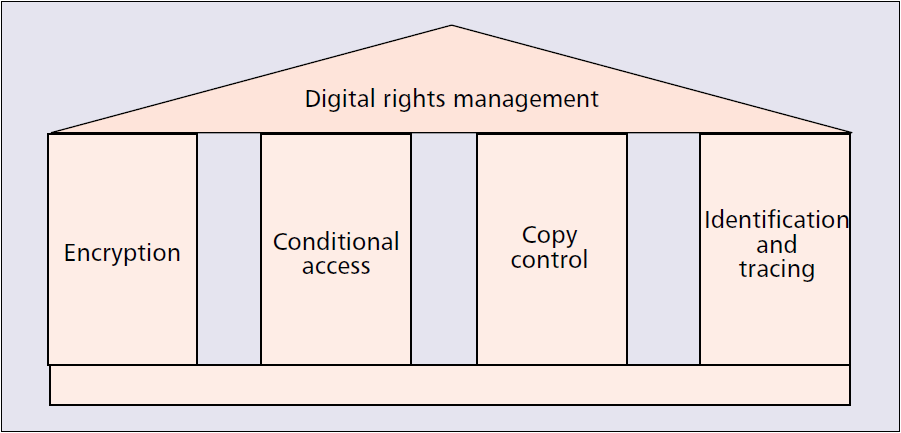
\includegraphics[width=13cm]{drm_pillar}
   \caption{The DRM pillar model (Copied from Hartung and  Ramme (2000) \cite{ieee:drm_watermark}).}
   \label{fig:def:drm_pillar}
\end{figure}

At large, as shown in figure \ref{fig:def:drm_pillar}, the DRM groups many technologies that will typically:
\vspace{-17pt} \begin{itemize} 
\item \textbf{Copy control}: Authenticate and identify the user and/or its devices to make sure the content is accessed and consumed by authorized person. 
\item \textbf{Encryption}: Protect and encrypt the content to avoid third party access.
\item \textbf{Identification and tracing}: Make each copy unique in order to identify them and track their usage.
\item \textbf{Conditional access}: Define and enforce the license such as if the user can copy the text, print it, limit the number of device that can access it, set the access duration (e.g. for library lending), if the copy can be shared and how many times, etc.
\end{itemize}

\begin{figure}[h]
   \centering
   	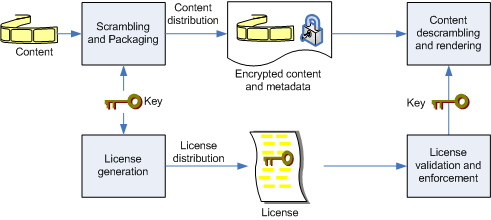
\includegraphics{indicare_drm}
   \caption{A generic DRM system (Copied from Bo\v{s}tjan Maru\v{s}i\v{c} et al. (2005) \cite{indicare:tiramisu}).}
   \label{fig:def:drm_scheme}
\end{figure}

A typical DRM content protection process is presented in figure \ref{fig:def:drm_scheme}. On the provider side, once the user purchases content, a key is associated to the user identity. The key will be used to sign the file to make the copy unique and protect the content with encryption (figure \ref{fig:def:drm_scheme}: \textit{Scrambling and Packaging}). In parallel, the usage contract (\textit{License generation}) is issued. After these steps, the encrypted content and the license are delivered to the user. On the user device, if the reading application is legitimate and will satisfy and enforce the license (\textit{License validation and enforcement}), the key is used to decrypt (\textit{Content descrambling}) the file and the content is now displayed to the user screen (\textit{Content rendering}). 

Even with strong encryption and full control on the software and hardware, there will always be ways to break any technical measure. To hamper software cracking to be implemented, distributed and used for protection removal, new articles have been added in the international copyright treaty to make cracking technologies illegal. 

Daniels \cite{dan:hard-soft-drm-1} use the term \textquotedblleft \textbf{hard DRM}\textquotedblright ~to describe the DRM system that restricts physical access and usage of the file. Rosenblatt ~\cite{idpf:lcp-uc} describes it as \textquotedblleft \textbf{heavyweight DRM}\textquotedblright. With that definition, he introduces the \textquotedblleft \textbf{lightweight DRM}\textquotedblright ~concept which is derived from the password-based encryption. With the \textbf{password protection}\label{def:password_protection} approach, there is no need to call back a distant server for authentication since the protection is embedded within the file. The key to decrypt the file is a password that the user has to enter before he can access the content. Like with hard DRM, this technique can also manage the authorization such as restricting printing or limiting copy of content. Usually, as there is no communication with a authentication server, this technology will not block concurrent access nor limit the number of devices which host copies of the file.

\section{Social DRM, Watermark and Fingerprint}

\textbf{Watermarking} and \textbf{fingerprinting} \label{def:watermark} are technologies used to identify a file. They originate from the information hiding techniques as presented in figure \ref{fig:def:drm_water_class}. Petitcolas et al. \cite{ieee:info_hiding} classify them as robust copyright marking if it is infeasible to remove them or if removing them will destroy the file at the same time. Otherwise, they classify them as fragile if the copyright marking is destroyed when the file is modified. 

\begin{figure}[h]
   \centering
   	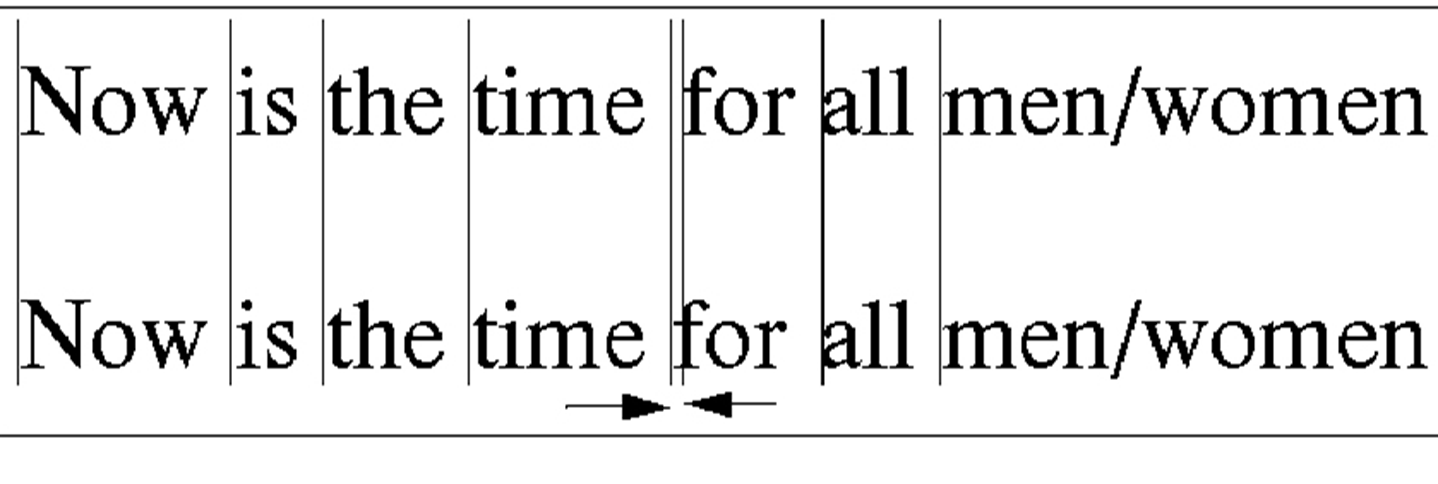
\includegraphics[width=9cm]{watermark}
   \caption{Word-shift watermark example (Copied from Insup Lee (2001) \cite{lee:watermark}).}
   \label{fig:def:drm_watermark}
\end{figure}

Watermark consists of data representing the user that are inserted and hidden inside the file bytes. For example, they can be imperceptible changes to the content such as spaces and invisible characters at the end of the chapter, modified pixels of the font, changes in the line/text spacing like in figure \ref{fig:def:drm_watermark}. One important aspect is the number of different watermark techniques used, so the cracker can never be sure to have defeated them all.

\begin{figure}[h!]
   \centering
   	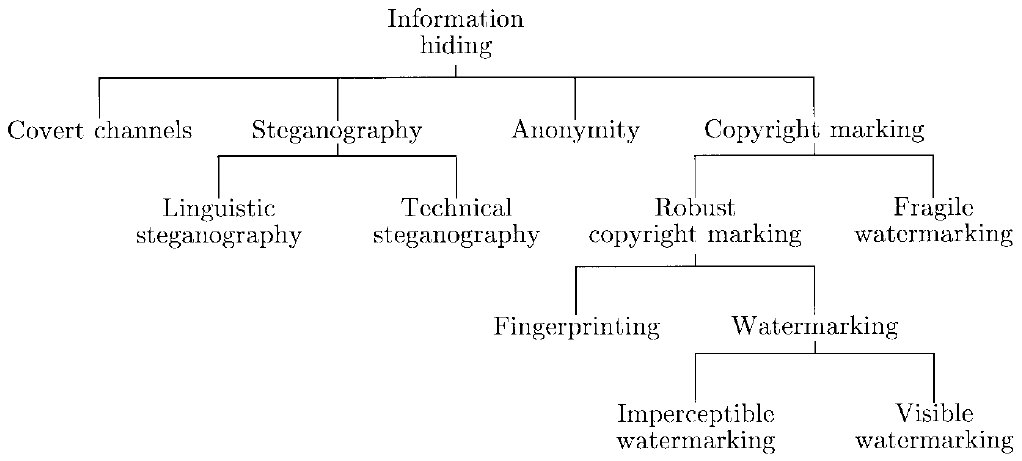
\includegraphics[width=11cm]{information_hiding}
   \caption{A classification of information-hiding techniques (Copied from Petitcolas et al. (1999) \cite{ieee:info_hiding}).}
   \label{fig:def:drm_water_class}
\end{figure}

Fingerprint is a technique only to identify a copy of a file by generating a cryptographic hash. With Watermark, these techniques can be used for a posteriori protection. Because identification does not control the permission, the user can do whatever he wants with the file. The idea is, if illegal content appears for example on a peer-to-peer network, to be able to find the user who did it.

A similar approach to watermarking is \textbf{social DRM}. The difference is that the information about the user is not hidden but visible. It can be for example part of meta-data or simply visible in plain text e.g. in the footer of every page. In figure \ref{fig:def:drm_socialDRM}, the PackaDRM\footnote{Packaged Digital Rights Messaging or PackaDRM\texttrademark ~ (\url{http://www.enthrill.com/pubtech})}  presents the user information in the \textquoteleft terms and conditions\textquoteright ~section of the e-book. The idea is to let the user do what he want but putting social pressure on him not to do anything illegal.
 
\begin{figure}[h]
   \centering
   	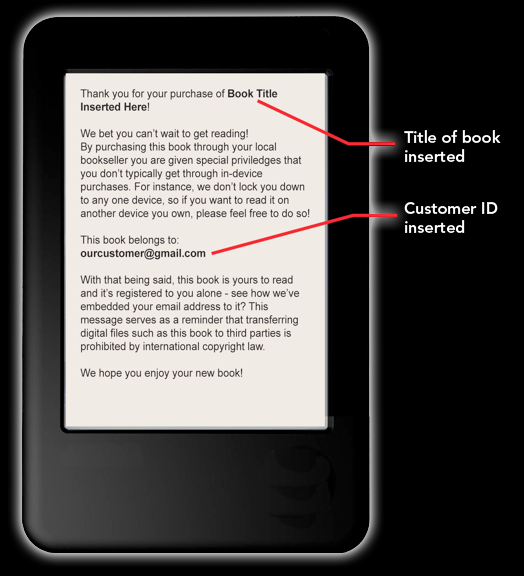
\includegraphics[width=11cm]{PackaDRM}%
   \caption{Social DRM (Copied from Kevin Franco (2012) \cite{kevinfranco:socialDRM}).}
   \label{fig:def:drm_socialDRM}
\end{figure}

The watermarking and all other identification techniques can and are often used in combination with the DRM. For example, Rosenblatt \cite{idpf:lcp-rfp} specifies that the Lightweight DRM \textquotedblleft is intended to be complementary to watermarking\textquotedblright . Hartung and Ramme \cite{ieee:drm_watermark} state \textquotedblleft watermarking [\ldots] is only useful as a system component, with the most important application being DRM and copyright protection in general\textquotedblright . Daniels \cite{dan:hard-soft-drm-2} refers to the combination of social DRM and watermark as \textquotedblleft\textbf{soft DRM}\textquotedblright ~because it does not restrict usage unlike DRM and still help in reducing copyright infringement, so \textquotedblleft better than no DRM at all\textquotedblright .

The task to find illegal copies of the work, whether it is protected or not, is usually devoted to crawlers as described in appendix \ref{app:crawl}.


\section{Law}\label{def:law}

In order to have effective protection and to make the crack illegal, the World Intellectual Property Organization\footnote{The WIPO is an United Nations (UN) agency established in 1967 which is responsible for the use of intellectual property (such as copyright, patents, trademarks, etc.) and count 185 member states (from: \url{http://www.wipo.int/about-wipo/en/}).} (WIPO) has added measures to protect DRM in its WIPO Copyright Treaty (WCT) of 1996 \cite[articles 11 and 12]{wipo:wct}. These articles are enacted in the European Union (EU) in the DIRECTIVE 2001/29/EC OF THE EUROPEAN PARLIAMENT AND OF THE COUNCIL of 22 May 2001 on the harmonisation of certain aspects of copyright and related rights in the information society \cite[chapter III]{eur-lex:2001/29/EC} implemented in Finland under the COPYRIGHT LEGISLATION of 2010 \cite[chapter 5a]{finlex:copyright_act}. Under the 89 WCT contracting parties such as China, Japan, Canada, Russian Federation, let mention the United States of America who enacted this treaty under the Digital Millennium Copyright Act of 1998 \cite[section 103]{gpo:dmca}. Notice also that countries such as India or Brazil are not signatories of the WCT.

\label{def:law_drm}In the WCT \cite[article 11]{wipo:wct}, EU DIRECTIVE 2001/29/EC \cite[article 6]{eur-lex:2001/29/EC} and Finnish COPYRIGHT ACT \cite[sections 50a and 50b]{finlex:copyright_act}, removing, circumventing any effective technological measures (such as hard and lightweight DRM), providing or producing tools to remove or circumvent it are prohibited. Finnish COPYRIGHT ACT  specifies that anyone who circumvent DRM, produce or distribute tool or device for circumventing a technological measure \textquotedblleft shall be sentenced [\ldots] to a fine for a violation of a technological measure\textquotedblright ~\cite[section 56e]{finlex:copyright_act} and \textquotedblleft shall be obliged to pay the author damages for any loss, mental suffering or other detriment caused by the crime\textquotedblright ~\cite[section 57(3)]{finlex:copyright_act}.

\label{def:law_watermark}The WCT \cite[article 12]{wipo:wct}, EU DIRECTIVE 2001/29/EC \cite[article 7]{eur-lex:2001/29/EC} and Finnish COPYRIGHT ACT \cite[section 50d]{finlex:copyright_act} make illegal to remove or alter right management information. They also make illegal to distribute, import for distribution, broadcast, communicate or make available to the public a work from which electronic rights-management information has been removed or altered. The Finnish COPYRIGHT ACT \cite[chapter 7, sections 56f and 57(3)]{finlex:copyright_act} specifies the same type of punishment as for circumventing a technological measure.

The the WCT \cite[article 12(2)]{wipo:wct} defines right management information as \textquotedblleft information which identifies the work, the author of the work, the owner of any right in the work, or information about the terms and conditions of use of the work, and any numbers or codes that represent such information\textquotedblright . To make sure that the social DRM belong to that definition, part of the social DRM should be placed in under the copyright notice or under the terms and conditions section of the e-book. Another solution could also be to have a book ID (which identifies the work) in different places in the e-book and to store that information with user purchase detail in reseller database. 

According to Rosenblatt \cite{rosenblatt:pottermore}, watermarking does not qualify as right management information. Even if the terms and conditions would state that removing the watermark is forbidden, \textquotedblleft it is possible that copyright law may prevail over such terms; this is a legal gray area\textquotedblright . Another problem with watermark that he raises is that \textquotedblleft a lightweight DRM that is susceptible to one-click crack has more protection than, say, a watermark removal tool\textquotedblright ~\cite{idpf:lcp-uc}. A watermark removal tool is legal because the watermark cannot be considered as an effective technological measure, while a DRM removal tool is illegal. This incomplete law protection could be one more argument to use watermark only in combination with other protection techniques or as Hartung and Ramme state \textquotedblleft watermarking is not a standalone technology\textquotedblright \cite{ieee:drm_watermark}.


Without technical protection, any work in electronic form still benefit from the copyright law. The author will continue to profit from the exclusive rights such as the protection for the usage and distribution of its work. With the ease of copying, modifying and sharing electronic content compare to the physical world, instead of fighting against the users, the author can surrender some of its rights for example allow non-commercial sharing and remixing. This waiving could be done for example by using a copyright license such as one of the Creative Commons\footnote{\url{http://creativecommons.org/}} licenses.



\chapter{Electronic Book (e-book)}\label{def:e-book}

According to Oxford Dictionaries~\cite{oxford:dictionary:e-book}, an \textbf{electronic book (e-book)} is \textquotedblleft an electronic version of a printed book which can be read on a computer or a specifically designed handheld device\textquotedblright . Unfortunately, this definition doesn't consider that some e-books do exist without theirs printed equivalent\footnote{such as Mile 81 from Stephen King \url{http://www.stephenking.com/promo/mile_81/}.}. The Cambridge Dictionaries~\cite{cambridge:dictionary:e-book} makes it clearer by defining it as \textquotedblleft a book that is published in electronic form\textquotedblright . They also add a second definition where the e-book term can be used for the hardware specific \textquotedblleft electronic device with a screen which allows you to read an electronic book\textquotedblright . Marshall \cite[section 2.4]{marshall:reading} completes the definition by including also the software/application needed to display the book on screen.

About the question of whether or not the physical books should have their electronic equivalent, Marc Levy (a best-selling French author) answered:
\begin{quote}
[Speaker:] You, the e-book scares you or seduces you?

[Marc Levy:] [\ldots] I think the e-book is a great opportunity for the book. Nobody can prevent the emergence of the electronic tablets [device]. If on the electronic tablet there is only video games, manga and television films, it means that on the entertainment platform there will be no books and within 20 years nobody will read any more.\footnote{My translation} \cite[from 13:45 to 14:28]{cplus:levy}
\end{quote}



\section{E-book File Formats and Protection}

For e-book there are different file formats available with their qualities and limitations.

The most basic file format is the plain text which has the advantage of being universal which means that it can be read on any operating system (OS), even in command line environment. They also can be compressed with an external tool for transport. This format was designed to display text only and do not offer formatting such as bold or italic text, makes impossible to insert images or interactive links, etc. And finally it offers no support for content protection; with administrator privilege, the end user can easily copy the full text and modify it. 

\label{def:e-book:pdf}In 2008, after seventeen years of existence, the portable document format (PDF) became a standard. It is a popular format on the internet for document exchange. For e-book, according to a 2012 French survey \cite[p. 19]{OpinionWay:baro_v1}, it is the preferred format for 53\% of the readers. By being a standard, every operating system can have application to display and print files in this format. PDF format was designed to be page oriented where the electronic version is the same as its print equivalent (this is sometimes seen as a problem, especially on small screen) but supports also re-flow feature. At the protection level, the author of the file can allow or deny the printing, copying of content, page extraction, etc. and the file can be secured by password or be electronically signed \cite{adobe:pdf}. 


\label{def:e-book:epub}Another open standard file format widely use for e-book is EPUB (short for electronic publication) standardized in 2007 which is the successor of the Open eBook (OEB) format of 1999 \cite{idpf:epub}. As of 2012 its latest version is EPUB 3. 

EPUB format uses web standards:
\vspace{-17pt} \begin{itemize}
\item Hyper Text Markup Language (XHTML (in EPUB 2) or HTML 5 (in EPUB 3)) files representing the text and structure.
\item Cascading Style Sheet (CSS) for the formatting.
\item eXtensible Markup Language (XML) for the navigation.
\item Additionally images, sounds, videos, etc.
\end{itemize}
\vspace{-17pt}	 
all together compressed into the EPUB file. 
This native compression is advantageous for the device disk usage and for faster transmission. 
The other big difference with the PDF is the use of the dynamic layout and pagination of the HTML so the text will be adapted on the fly to the display area and the user preferred font size \cite{idpf:epub3}. 


\label{def:e-book:epub-drm}The EPUB file format offers a protection layer but \textquotedblleft does not specify a required format for DRM\textquotedblright ~\cite[section 2.5.5]{idpf:ocf_spec}; so the choice is in the hands of the vendor. As example, the Adobe DRM can be use to protect EPUB files. Actually, the International Digital Publishing Forum (IDPF)\footnote{IDPF is the organization responsible to maintain the EPUB standard.} is proposing \textquotedblleft requirements for a potential content protection scheme for EPUB\textquotedblright ~\cite{idpf:drm-rfc}, the lightweight DRM.

\label{def:e-book:iba:azw}
In 2000 Mobipocket.com developed its own e-book file format as part of their MobiPocket Reader application. This format, like ePub, is based on the Open eBook (OEB) specifications. The file can be natively secured with their solution but also left unencrypted. Mobipocket became part of Amazon in 2005 \cite{mobi:about}.

After Amazon acquisition, they build their own protection on top of the Mobipocket format (with a .azw extension). This has made the future of the protected .mobi e-book unclear \cite{tdr:rip_mobi} while unprotected .mobi files can still be read from Amazon Kindle devices as well as many reading applications. Amazon also announced the creation of their new Kindle Format 8 based on HTML 5 and CSS 3. Like the .azw, it can be protected with Amazon DRM. This format should continue to be backward compatible with Mobipocket. The Amazon e-books file format can be read from Amazon Kindle devices or with Amazon OS-specific Reading apps\footnote{\url{http://www.amazon.com/gp/feature.html?ie=UTF8&docId=1000493771}}  \cite{amazon:kf8}. 

Apple also has its own e-book file format (iBooks) based on EPUB 3 but with their own mimetype and proprietary CSS extensions \cite{glaz:iba}. The e-books in this format can be protected by Apple DRM and if obtained through their store, it will anyway be watermarked. This format is designed to be only readable with the iBooks application\footnote{\url{https://itunes.apple.com/us/app/ibooks/id364709193?mt=8}} and only on Apple mobile devices. For an author/publisher, the only way to sell e-books in this format is through the Apple store \cite{apple:iba_faq}.

\section{E-book Applications}

For e-book, at the application level, there are three categories of software. First to create an e-book, even if some writers will still hand or typewriting their text, it is common that they use a computer with a basic text editor\footnote{such as notepad} or a word processor\footnote{such as Microsoft Word (\url{http://office.microsoft.com/en-us/word/}) or OpenOffice.org Writer (\url{http://www.openoffice.org/product/writer.html})}. The editor then formats the text with a typesetting\footnote{such as \LaTeX (\url{http://www.latex-project.org/})} or a publishing\footnote{such as Adobe InDesign (\url{http://www.adobe.com/products/indesign.html})} or a WYSIWYG\footnote{WYSIWYG stands for What You See Is What You Get} editing\footnote{such as Sigil (\url{http://code.google.com/p/sigil/})} software to generate the e-book file and its metadata. 

Nowadays, some vendors propose the same e-book in different file formats to offer the reader with a greater choice of devices, operating systems and reading applications where the e-book can be read.
While some of the edition software can generate the e-book in different files formats, it also can be done with a conversion software\label{def:e-book:app:calibre}\footnote{such as Calibre (\url{http://calibre-ebook.com/}) or Pandoc (\url{http://johnmacfarlane.net/pandoc/})}. Sometimes, such conversion is done by the reader himself if he cannot read his e-book on a specific device or with his preferred reading application.

Finally, to read the e-book file, the end user will need a software that will display the e-book on the device screen. Marshall \cite[chapters 3, 4 and 5]{marshall:reading} state that these reading applications should at least provide the same functionalities as what can be achieved with a physical book, such as:
\vspace{-17pt} \begin{itemize}
\item Navigating, moving to the next/previous page, going to a specific page/chapter, etc.
\item Keeping the user oriented, where he is in the book and how much left (page number out of the total).
\item Annotating, that can be simple as a bookmark, line mark that the reader can use to quickly navigate to a specific part of the e-book (for example to remember where he stopped reading to restart reading from there); highlighting; a comment about a sentence, paragraph, chapter, the all e-book; a summary or a description of the e-book or part of it; etc. ~\cite{w3c:uc_annotation}
\item Printing.
\item Clipping, like copy-pasting an extract for quotation, etc.
\item Social interaction, like sharing annotations, etc.
\end{itemize}
\vspace{-17pt}
She describes these functionalities as the \textquotedblleft live-or-die aspects of the electronic book\textquotedblright ; not having them \textquotedblleft ensures that readers will reject eBooks [in the largest sense (the electronic reading as a all)] out of hands\textquotedblright .

Some others interactions that can be done with a physical book and that should be available with an e-book do not necessary depends on the reading application. In these activities there are the acts of buying or borrowing,  some parts of the social reading such as sharing quotes and comments and the actions of offering, lending, sharing, swapping, crossing or reselling an e-book.

In addition to the printing equivalent, the electronic book application offers extra features. Marshall \cite[chapter 7]{marshall:reading} gives examples like:
\vspace{-17pt} \begin{itemize}
\item Searching, for example entering a keyword that will indicates the location of all the occurrences in the text and providing links to the found results
\item Linking that can be used to facilitate the navigation within the book, like clicking on one item in the table contents to move to a specific chapter or from a searched result, etc. And can also be used to refer to external resources, for example to a web page that contains extra information, etc.
\item The possibility to automatically translate the text into another language.
\end{itemize}
\vspace{-17pt}
She also points the advantage that with a devices which can store many files, the reading application could offer searching facilities at the collection level and the use of metadata to better organize and find  content within the library. The metadata can be from the book itself (like title, author, etc.) or user based (both implicit (what was read and when) and intentional (annotations)).

With new technologies, the e-book can be enriched with multimedia elements like sounds or video and thus gives more interaction to the reader. With internet connected devices (if the user store its library on-line and if the reading application is synchronized) the reader can start reading in the train on his mobile phone and continue reading on his computer once at home. Some reading application offers also text to speech feature via a speech synthesizer that reads the text aloud.

With e-book, the user behaviour can more easily be studied with analytical tools. The user can then know when, where and how fast he reads. Such type of information can be of high value for researchers and also for publishers who can study what the user likes most and can use this to propose similar contents to the reader.

Part of the e-book interactions described in this chapter are presented as use cases in annex \ref{ebook:uc}

\section{E-book Devices}

At the hardware level, the minimum required to display an e-book is a device with a screen and input capability. A reader can use a computer, laptop, smart-phone, tablet or dedicated e-reader device. The dedicated e-book reading device offers numerous advantages comparing to the others, such as cheap prices and a good reading ergonomic: adapted controls, light weight, electronic ink (E-Ink) screen, etc. \cite{about:ipad}.

E-Ink offers comfort for reading in full sunshine \textemdash which can be hard with the other type of devices due to the brightness and contrast of their screen\textemdash as well as in the shadow. This screen technology consumes very few battery giving a very long autonomy in weeks compare to days or hours of other mobile devices. Once displayed on E-Ink screen, the text will stay forever while the others types of screen will usually shut down to save energy which can be very annoying for reading. 
The new E-Ink device, such as the Kindle Paperwhite\footnote{\url{http://www.amazon.com/gp/product/B008GEKXUO/ref=fs_cl}} are back lighted, allowing to read in the night. Older ones require an external source of light.
Even if E-Ink prototypes with color have been demonstrated\footnote{\url{http://www.geek.com/articles/gadgets/e-ink-promises-thinner-lighter-higher-resolution-and-color-e-paper-displays-2011095/}}, they offer a small palette compare to the full range of colors of the other type of devices. And currently, on the market, most of the e-book reader are still black and white with shade of grey.


Another problem with e-book devices is that they usually only have an indirect internet access trough WLAN\footnote{Wireless Local Area Network} or no access at all forcing the user to physically connect the device to a computer for loading the e-book files. This problem also applied to some tablets and laptops, for example if a Wi-Fi\footnote{Wireless connection} access point is not present. However, the connection through the mobile network antenna would require a UMTS/LTE\footnote{UMTS (Universal Mobile Telecommunications System) and LTE (Long Term Evolution) are the new generation of GSM (Global System for Mobile Communications) cellular networks system and offer access to Internet through it.} subscription which has a cost.

The advantage of being specific for e-book reading can also be seen as an inconvenient. For example, if the user would need dedicated hardware to perform every other activities, such as watching films, playing games, etc., he would need to travel with a lot of different devices. Another difficulty shared with smart-phone is the small disk capacity of the early versions of these devices that is nowadays increasing and limiting this problem. Except for the mobile phones that are smaller and lighter, the e-reading devices are the most convenient for transport compared with tablet and laptop.



\chapter{Existing and Upcoming Protection Technologies}\label{exist}

\section{Existing E-book DRM Systems}

Nowadays, there are four major e-book DRM systems in use: Adobe, Amazon, Apple and Marlin Trust Management Organization (MTMO)\footnote{\url{http://www.marlin-community.com/technology/how_marlin_works}}. Nook DRM system is based on Adobe solution. 

Fifth major system, the Microsoft e-book DRM technology cannot be considered in use since it was part of the Microsoft Reader that has been discontinued in August 2012 (see section \vref{def:opp_ms}). Microsoft will probably use their PlayReady\footnote{\url{http://www.microsoft.com/playready/}} technology to protect e-book. Their white paper specifies that  \textquotedblleft Microsoft PlayReady supports essentially any type of content, including games, images, and ringtones, in addition to music and video.\textquotedblright ~\cite[p. 4]{ms:playready}; but don't explicitly have the e-book in the list. 

\subsection{Adobe DRM in Detail}\label{def:adobe_drm}

Adobe e-book DRM, namely Adobe Digital Experience Protection Technology (ADEPT), is part of their platform which is centred on the Adobe Content Server (ACS)\footnote{\url{http://www.adobe.com/products/content-server.html}}. ACS serves as both hosting and managing PDF and EPUB e-books distribution and encryption. Finally, to access the protected content, the user will use the Adobe Digital Editions\footnote{\url{http://www.adobe.com/products/digital-editions.html}} software for Windows or Mac, or an application written with the Adobe Reader Mobile Software Development Kit (SDK)\footnote{\url{http://www.adobe.com/devnet/readermobile.html}} for e-reader device, tablet or smart-phone \cite{adobe:whitepaper}. The figure \vref{fig:def:adobe_workflow} shows the flow of authoring and delivering an e-book with Adobe solution.
\begin{figure}[h]
   \centering
   	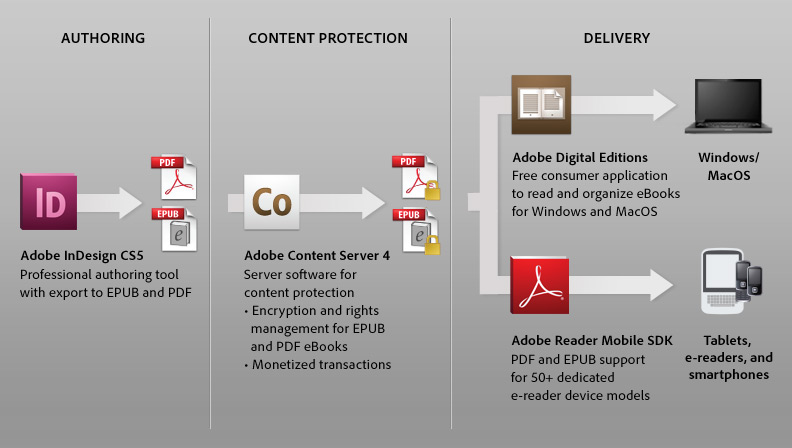
\includegraphics[width=14.7cm]{adobe_ebook_workflow}
   %
   \caption{Adobe Digital Publishing Solution for eBooks (Copied from Adobe (2012) \cite{adobe:digital_publishing}).}
   \label{fig:def:adobe_workflow}
\end{figure}


In the normal flow (see figure \vref{fig:def:adobe_cs}), the user visits the publisher or retailer web store to buy an e-book. After the purchase confirmation, he will receive an Adobe Content Server Message (.acsm) file and by opening it with the Adobe Digital Editions, the software will communicate online with the Content Server that will encrypt the e-book and provides it DRM protected with the publisher’s authorizations for the user based on his adobe ID. Before the user can read the e-book, he must also have registered his device. That way, the platform makes sure that the file owned by the user is not distributed further. 
\begin{figure}[h]
   \setlength{\fboxsep}{3pt}
   \fbox{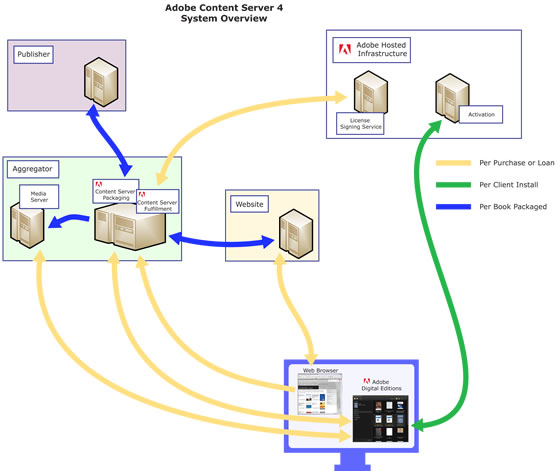
\includegraphics[width=14.7cm]{adobe_cs4-overview}} 
   \caption{Adobe Content Server Architecture (Copied from Adobe (2012) \cite{adobe:content_server_architecture}).}
   \label{fig:def:adobe_cs}
\end{figure}
 

Adobe DRM system allows the user to register up to 6 devices, so the user can access his library, annotations, bookmarks, etc. on all of them, e.g. start to read on his e-reading device, continue on his smart-phone and finish on his laptop. This can also cover the family fair use where people share a home computer.

\subsection{Advantages and Limitations of Adobe DRM}

One natural thing that user can do with physical books is to share it with friends. 
Unfortunately, DRM do not allow it since the e-book is protected for the user and its devices only. 
In order to give sharing facility Adobe offers another way to provide the e-book to the user with a password-only protection \cite[Ability to share section]{adobe:whitepaper}. The password will be encrypted with the file and it will be impossible to modify it. The publisher can choose to let the user define it and allow an open sharing or use a social DRM like approach where the publisher create the password for the user (e.g. using user credit card number, email address, etc.) to refrain the user to share it worldwide. This password-only protection option is without Adobe DRM; so the file can either be DRM protected or password protected but not both. 

An advantage of Adobe e-book DRM when compare to Amazon and Apple is that the user is not \textquotedblleft imprisoned in a walled-garden system\textquotedblright ~\cite[Open environment section]{adobe:whitepaper} and can purchase DRM protected e-books and/or borrow from different vendors/libraries and can aggregate, organize and read them within the same application. Apple iBookstore allows only iOS devices to purchase files from their store and also prevent them to get e-books from a retailer who use a different DRM in their iBooks application. And to finish the Apple close loop, e-book created from their iBooks Author tool can only be sold through iBookstore \cite{zdnet:apple_ibooks_license}. Amazon Kindle device also lock the user with a single vendor. But Adobe argument is that many vendors use their DRM making the multiple vendors aggregation possible; but the Adobe Digital Editions will not allow opening an e-book encrypted with another DRM.

For publishers and authors, another advantage of Adobe DRM approach is the use of the open and well known formats PDF and EPUB, in opposition to the proprietary format from Apple iBooks and Amazon Kindle, thus simplifying the production, publication and distribution process \cite[How the Adobe eBook Platform helps publishers section]{adobe:whitepaper}. For the reader however, the advantages of these open formats get reduced. As an example, the DRM force the user to use an Adobe authorized software, preventing him to use his favourite EPUB/PDF reading application and can thus create some confusion.

Another claim of the Adobe whitepaper \cite[Device interoperability section]{adobe:whitepaper} is the possibility to read DRM protected e-books on multiple platforms. In fact, Adobe provides only the computer support with their free\footnote{Free here has the meaning of gratis/no price.} Adobe Digital Editions application for Windows and MacOS Operating systems, excluding GNU/Linux \cite{adobe:ade_linux}. For other devices, a third party has to develop a dedicated application using the Adobe Reader Mobile SDK, for which they have to pay a licence. Even that the price is fixed on a case-by-case basis, this can be unfair for a small publisher and is seen as another way from Adobe to monetise their DRM. 


On the Adobe price politic, in 2008, the license for the Adobe Content Server was \$5000\footnote{United States dollar (USD)} plus an extra \$1500 per year for the support, maintenance, upgrade and the access to the Digital Signing Service \cite{adobe:content_server_price}. And in 2012, from the Adobe Technology Partner in Europe \cite{ctrlpublishing:content_server_price}, the license is \$8000 plus \$2000 per year support. They also charge \$2495 for the installation and configuration. On top of that price, signing one e-book permanently will cost \$0.22 (\$0.08 for a 0-60 day expiring (e.g. for a library lending)). If such price is affordable for a big publisher, it can be too much for a small one.
\begin{figure}[h]
   \setlength{\fboxsep}{3pt}
   \fbox{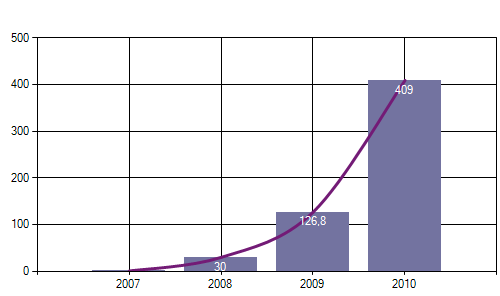
\includegraphics[width=14.1cm]{e-book-sales-finland}}
   \caption{Downloaded e-books total. Yearly sales (1000 \euro) 2007-2010 in Finland. 
   (Copied from Finnish Book Publishers Association (2012) \cite{kustantajat:year_sale_ebook}).}
   \label{fig:def:e-book-sale-fi}
\end{figure}

As example,\label{def:e-book-sale-fi} based on the yearly sales in Finland (see figure \ref{fig:def:e-book-sale-fi}), it can be reasonable to say that a publisher sell ten thousand e-books per year. If he want to cover the license and installation (e.g. over a three year period) price, the yearly fee plus the 22 cents per e-book, he would have to charge an extra \$0.77 per e-book he sell (and that do not include other charges for maintaining a server (like hardware/software installation and maintenance, electricity, domain name and internet address, etc.)). 

It is not possible for a user to offer or resell his e-books. Due to the fact that the DRM is associated to the user and the device, it will be hard to try to read an e-book on a public computer (e.g. in an internet coffee). Also, if the user reach the limit of the 6 registered devices, buy a new computer and want an old one to be unregistered to replace it with his new one, he will face a long procedure to do so.

About two year after the release of the Adobe Digital Editions the explication on how to circumvent the Adobe ADEPT DRM was published on the I$\heartsuit${\footnotesize CABBAGES} %\textsc{cabbages}
 blog\label{def:adobe_drm_crack} \cite{icabbages:adobe_drm_hack}. The author specifies that the Adobe file encryption was strong but the weakness was in how the Adobe Digital Editions hide the key. Nowadays, there are companies like epubor\footnote{\url{http://www.epubor.com/adobe-digital-editions-ade-drm-removal.html}} that do business by selling DRM removal tools.
 
%\section{Technical Implementation of Lightweight DRM}

%TODO:\\
%- different hash for password and content. (avoid hash=hash crack but still subject to brute force,  Rainbow table or social crack).\\or how to hide pwd hash?\\
%- local signing app V.S. DRM vendor web service \\
%- client-server interaction?



%http://stackoverflow.com/questions/822468/is-there-an-open-source-drm-solution
%http://www.w3.org/2000/12/drm-ws/pp/iprsystems-iannella.pdf
%http://www.roseindia.net/opensource/open-source-drm.shtml
%http://www.numerama.com/magazine/1672-un-standard-drm-industriel-open-source.html

%http://www.gnu.org/licenses/gpl-faq.html#DRMProhibited

%TODO...\\
%- Marlin DRM (hybrid approach)\\
%- idpf lightweight protection (and my participation)\\
%- w3c protection (almost no hope?)\\
%- ...

\section{DRM Encryption Pillar Using W3C Standard}

This work research if a DRM system could be made to protect an e-book while at the same time reduce the restriction to the fair use. Currently, one drawback of the DRM system is the lack of interoperability, like the impossibility to read an e-book on different platform. This chapter will test if the possibly upcoming W3C Web Cryptography API\footnote{\url{http://www.w3.org/TR/WebCryptoAPI}} standard could be used for the protection and encryption part of such DRM system.

The assumption is that most of the modern devices do or can have a JavaScript capable web browser and can be connected to internet directly or through another device. If asserted, then making a web based DRM system where the user could use his favourite browser on any device to read protected content could offer a better interoperability than most of the existing DRM systems.

The idea to make part of a DRM system with the Web Cryptography API originates from the W3C Use Cases~\cite{w3c:uc_webcrypto} such as the \textquotedblleft Banking Transactions\textquotedblright ~where a user uses a public and private cryptographic key pair to exchange messages that he will be the only one able to read and the \textquotedblleft Authenticated Video Services\textquotedblright ~use case where the user get encrypted content from a distant service over the internet that only his device can display.

With the Web Cryptography API being in the draft state and with most of the exiting browsers having only a partial implementation of it\footnote{\url{http://www.w3.org/2012/webcrypto/wiki/Main_Page#First_implementations}},
the PolyCrypt\footnote{\url{http://polycrypt.net/}} implementation is used as a fall-back. That library tests and exposes the needed cryptography libraries if not yet implemented natively by the browser. 

The starting point for the code is the web-crypto-samples application\footnote{\url{https://github.com/nvdbleek/web-crypto-samples}}, Copyright (c) 2013 Nick Van den Bleeken under MIT License. The file \url{base64.js} is an exact copy from this application, used as a library. Part of his \url{utils.js} and \url{encrypt.js} scripts are derived into the \url{keydecrypt.js} code as seen in annex \ref{source:code}.

\subsection{Technical Implementation Using Web Cryptography API}

As a first step, this application, generate the public and private key pair on the client side if they do not exist. This operation correspond to the KEYGEN-ASYM requirement of the W3C Web Cryptography API Use Cases~\cite[chap. 2]{w3c:uc_webcrypto}. The listing \ref{js:genkey} shows the JavaScript code used to generate the 2048 bits keys (lines 1 to 7) with the Public-Key Cryptography Standards (PKCS) RSA algorithm and the callback method if the keys get generated successfully (lines 9 to 17). After creation, the keys are stored on the user computer (lines 13 and 14) for later cryptographic operations.

\vspace{-12pt}\begin{lstlisting}[language=JavaScript,caption={Generating public and private cryptography key pair},label=js:genkey]
var genOp = webCrypto.generateKey({
	name : "RSAES-PKCS1-v1_5",
	params: {
		modulusLength : 2048,
		publicExponent : new Uint8Array([ 0x01, 0x00, 0x01 ])
	}
}, true, [ "encrypt", "decrypt" ]);

//the onerror callback function is not shown here

genOp.oncomplete = function(e) {
	publicKey = e.target.result.publicKey;
	privateKey = e.target.result.privateKey;
	if(publicKey && privateKey){
		localStorage["fi.metropolia.key.public"] = JSON.stringify(publicKey);
		localStorage["fi.metropolia.key.private"] = JSON.stringify(privateKey);
		//... here comes exporting keys code ...
	}
}
\end{lstlisting}\vspace{-12pt}

If the user keeps the private key secret and shares the public key, he makes sure that he will be the only one to be able to decrypt and read the content encrypted with his public key, since only his private key can do this decryption. Since the raw public key is not suitable for the sharing process, it will first be converted into the JSON Web Key (JWK) format\footnote{\url{https://tools.ietf.org/html/draft-ietf-jose-json-web-key-25}} as shown in the listing \ref{js:export}. This operation correspond to the EXPORT requirement of the W3C Web Cryptography API Use Cases~\cite[chap. 2]{w3c:uc_webcrypto}.

\vspace{-12pt}\begin{lstlisting}[language=JavaScript,caption={Exporting public key},label=js:export]
//Export the public key
var exportOp = webCrypto.exportKey("jwk", publicKey);

//the onerror callback function is not shown here

exportOp.oncomplete = function(evt) {
	//stringify the JWK public key
	var n = JSON.stringify(evt.target.result);
	//key ready to be shared
	document.getElementById('public_key').innerHTML = n;
}
\end{lstlisting}\vspace{-12pt}

After the exporting preparation operation, the user sends his now ready public key to the server which will use that key to encrypt the content specifically for him. But before encryption, the server will first import the key as presented in the PHP code of listing \ref{php:import}. This operation correspond to the IMPORT requirement of the W3C Web Cryptography API Use Cases~\cite[chap. 2]{w3c:uc_webcrypto}. With no PHP function found to import the JWK format strait, the key is first converted into the X.509 Privacy-enhanced Electronic Mail (PEM)\footnote{\url{https://tools.ietf.org/html/rfc2510}} certificate format.

\vspace{-12pt}\begin{lstlisting}[language=PHP,caption={Importing public key},label=php:import]
//receive the JWK key from the client
$pub_key = $_POST["public_key"];
$key_elem = json_decode($pub_key, true);
//convert the public key to PEM format
// dirty hack since it works only with a 2048 bits key 
// (hard coded headers)
//from http://fi1.php.net/manual/en/function.openssl-pkey-get-public.php#104439
$prepa = wordwrap('MIIBIjANBgkqhkiG9w0BAQEFAAOCAQ8A'.'MIIBCgKCAQEA'.str_replace(array("_", "-", "="), array("/", "+", ""), $key_elem["n"]).'ID'.$key_elem["e"], 64, "\r\n", true);
$key = <<<EOF
-----BEGIN PUBLIC KEY-----
$prepa
-----END PUBLIC KEY-----
EOF;
//import the key
$res = openssl_pkey_get_public($key);
\end{lstlisting}\vspace{-12pt}

With the public key successfully imported, the server is ready for the encryption process. The PHP script will first get the content of the uncompressed EPUB file stored in folder not accessible from internet as seen in the annex \ref{source:code} encrypt.php source code file. With a maximum of 1968 bits long string that can be encrypted with the 2048 bits long key, the content of the file to be encrypted is chunked  into pieces of 123 characters ($123 \cdot 16 = 1968$) and each of the substring get encrypted individually as shown in the listing \ref{php:encrypt}. This operation correspond to the ENCRYPT-ASSYM requirement of the W3C Web Cryptography API Use Cases~\cite[chap. 2]{w3c:uc_webcrypto}.

\vspace{-12pt}\begin{lstlisting}[language=PHP,caption={Encrypting the content of a file with the public key},label=php:encrypt]
//the file with the encrypted content
$write_file = "EPUBfolder/OPS/".$list_of_content[$current_file];
$resfile = fopen($write_file, "w");
//reading and encrypting 
foreach(str_split(file_get_contents("../../secret/EPUBfolder/OPS/".$list_of_content[$current_file]),123) as $val){
	openssl_public_encrypt($val, $encrypted, $res); //$res is the imported key
	fwrite($resfile, base64_encode($encrypted));
}
fclose($resfile);
echo "Encrypted file: <a href=\"$write_file\" target=\"_blank\">$write_file</a>";
\end{lstlisting}\vspace{-12pt}

Now that the content is specifically encrypted for him, the file can be sent to the user. To decrypt the content of the file, the JavaScript will use the use the private key. This operation correspond to the DECRYPT-ASSYM requirement of the W3C Web Cryptography API Use Cases~\cite[chap. 2]{w3c:uc_webcrypto}. The listing \ref{js:decrypt} present the code that decrypt the content of the file bloc by bloc asynchronously.

\vspace{-12pt}\begin{lstlisting}[language=JavaScript,caption={Decrypting content with the private key},label=js:decrypt]
var alg = { name : "RSAES-PKCS1-v1_5" };
var privateKey = JSON.parse(localStorage["fi.metropolia.key.private"]);
//decrypt the data bloc by bloc asynchronously
for(i = 0; i < blocData.length; i++){
	(function(closureI){
		decryptOp[closureI] = webCrypto.decrypt(alg, privateKey, new Uint8Array(Base64Binary.decodeArrayBuffer(blocData[closureI])));

		//the onerror callback function is not shown here
		
		decryptOp[closureI].oncomplete = function(evt) {
			resultArray[closureI] = ab2str(evt.target.result);
		};//decrypt
	})(i) //closure
}
\end{lstlisting}\vspace{-12pt}

Finally, with the asynchronous decryption process, all the decrypted parts are reordered and written in a local JavaScript blob object to be rendered to the user as shown in the listing \ref{js:render}. In order to get the image and styling associated with the EPUB XHTML pages, the URL are overwritten to let the browser getting the CSS and images files on internet.

\vspace{-12pt}\begin{lstlisting}[language=JavaScript,caption={Decrypting content with the private key},label=js:render]
function decryptedToBlob(){
	//hack to transform relative path to absolute hard-coded URL.
	var tmp = [];
	var j, hack;
	for(var i = 0; i < resultArray.length; i++){
		tmp = resultArray[i].split("=\"");
		if(tmp.length > 1){
			hack = "";
			for(j = 0; j < tmp.length - 1; j++){
				hack += tmp[j] + "=\"";
				if((tmp[j].endsWith("href") || tmp[j].endsWith("src")) && !tmp[j+1].startsWith("http://") && !tmp[j+1].startsWith("#"))
					hack += "http://hardcoded.fi/EPUBfolder/OPS/";
			}
			hack += tmp[j];
			resultArray[i] = hack;
		}
	}
	//array to blob to be used as the iframe source.
	var blob = new Blob(resultArray, {type : 'application/xhtml+xml'});
	document.getElementById("decrypted_blob").src = URL.createObjectURL(blob);
}
\end{lstlisting}\vspace{-12pt}

Part of the source code is listed into the annex \ref{source:code}.
 The \url{genkey_and_export.html} and \url{keydecrypt.js} representing the client side of the application responsible for the local operation of generating the keys, exporting the public key, decrypting the content with the private key and rendering the result to the user. The \url{encrypt.php} file represent the server side of the application responsible for importing the user public key and encrypting the content. The source code files that are not listed in annex \ref{source:code} are the non-modified files used as library, namely the PolyCrpt\footnote{\url{https://github.com/polycrypt/polycrypt/tree/master/src}}, Copyright (C) Raytheon BBN Technologies Corp, 2013, published under BSD 3-clause license\footnote{\url{https://github.com/polycrypt/polycrypt/blob/master/license.txt}} and the \url{base64.js}\footnote{\url{https://github.com/nvdbleek/web-crypto-samples/blob/master/js/lib/base64.js}} file , Copyright (c) 2013 Nick Van den Bleeken under MIT License\footnote{\url{https://github.com/nvdbleek/web-crypto-samples/blob/master/LICENSE}}.
 
A demonstration of this application is running at
  \url{http://users.metropolia.fi/~patricka/wcrypt-book/genkey_and_export.html} and the source code is available at the same place or in github\footnote{\url{https://github.com/patrick-ausderau/WebCryptoAPI}}. This software is licensed under the  GNU General Public License as published by the Free Software Foundation, either version 3 of the License, or (at your option) any later version. This application encrypt the public domain EPUB book Moby-Dick; or, The Whale by Herman Melville for the sole purpose of demonstration; the e-book originate from Project Gutenberg\footnote{\url{http://www.gutenberg.org/ebooks/2701}} where it is freely available.


\subsection{Known Problems and Possible Improvements}

With this application, the protection is only guaranteed during the transport between the server and the client machine. Once on the client machine, it is very hard to hide the private key and obfuscate the JavaScript decryption code. If the user retrieve the private key, he could write an alternative decryption application that could for example save unencrypted copy of the files that he could later share. With the JavaScript being an interpreted language, the reverse engineering process to modify the decryption code would be easier than with compiled language.

Currently, once decrypted, the content can easily be copied. But even if the selecting, copy-pasting and the print screen would be disabled, the user could still take physical picture of the content to save an unencrypted version of the text.

Another concern with JavaScript as stated by Matasano Security \cite{matasano:js_bad_crypto}, Matthew Green \cite{green:js_bad_crypto} or the PolyCrypt\footnote{\url{http://polycrypt.net/}} team itself is that this programming language and the current implementation of the Web Cryptography API can not be use for serious cryptographic operation. The language will suffer from many flaws such as \textquotedblleft side-channel attacks\textquotedblright , problem with the garbage collector where \textquotedblleft secrets are lurking in memory potentially long after they're needed\textquotedblright ~and many more. So at best, secure JavaScript cryptography could be possible only after it would be natively implemented and solidified by browser and seriously reviewed.

This application use the asymmetric decryption operation intensively and this operation is rather slow with the current implementation of the Web Cryptography API. A possible improvement would be to only encrypt part of the file, for example the first and last three paragraphs of each chapter, that would be enough to make the content unusable. Another option would be to use the asymmetric keys only to exchange symmetric session keys, as proposed by the use case \textquotedblleft Authenticated Video Services\textquotedblright~\cite{w3c:uc_webcrypto}, with the symmetric decryption being much faster.

Some possible improvements for this application would be to use the off-line storage provided by the HTML5 language, so the full encrypted content could be stored on the user computer to be read without internet connection and also making possible to do the decryption of the next chapter in the background so the user will not have to wait. The content, once decrypted could be better presented to the user, for example by using the \url{epub.js}\footnote{\url{https://github.com/futurepress/epub.js}} script. One know bug of this application is with the encryption and decryption of some special typographical characters such as the curly quotation marks or the em dash.



\section{Lightweight DRM}\label{def:idpf_light}

The DRM systems suffer from many drawbacks such as interoperability problem where the reader is limited to a single platform, the requirement to be connected to internet in order to be authenticated, the risk to loose his content if the vendor goes bankrupt, etc. This chapter explore the possible upcoming standard for a Lightweight DRM proposed by the IDPF and its attempt in limiting the DRM problems.

The Encrypted Media Extensions possible standard from the W3C was also scouted but quickly dropped because it will not be suitable for e-books. It is specifically designed for media elements\footnote{\url{http://www.w3.org/TR/encrypted-media/#extensions}}, namely video and audio files embedded or streamed into web pages.

\subsection{Lightweight Content Protection (LCP)}

In May 2012, IDPF made a proposal for standardizing a Lightweight Content Protection (LCP) that will be \textquotedblleft occupying a middle ground between strong DRM and DRM-free\textquotedblright ~\cite{idpf:drm-rfc} to protect EPUB e-books. The idea is to have a protection that will be strong enough to qualify as an \textquoteleft effective technical protection measure\textquoteright ~to benefit the law protection to guarantee the publisher/vendor with a full protection mechanism and at the same time to reduce the \textquoteleft hard DRM\textquoteright ~drawbacks \cite{idpf:lcp-uc}. 

The LCP will work as follows: when a reader acquires an e-book, the content (texts, images, etc.) will be protected with a password encryption and the hash of the password will be associated with the file and/or the reading application. To read the e-book, the user will be prompted to enter it the first time before accessing the content. Since the password cannot be changed and will be set at purchase time, it can be defined by the vendor/publisher (to be e.g. the reader full name, email address, credit card number, etc.) \cite{idpf:lcp-uc}.

With the password protection, there is no need to communicate with an authentication server, so LCP will work offline and it also means that the reader will really own the e-book (as long as he remembers the password) even if the provider ceases its activities. He will also have the freedom to have copies of his e-books on any devices he owns without limitation. The reader will be able to share his e-book; but will have to communicate the password too, so limiting him to people he trusts (friends/family) and refrain him to over-share it. Finally LCP will better respect user privacy by not spying the reader usage \cite[Why Consider LCP for EPUB? and What Is LCP? sections]{idpf:lcp-uc}. 

With the content encryption, the publisher/vendor can also define limitation on usage like printing, copy of content, editing, etc. There will be also a possibility to set an expiration date which can be interesting for library lending. Basically, the provider will be able to set the same type of protection that he can do with other DRM \cite[EPUB LCP Requirements section]{idpf:lcp-uc}.

By lightweight, it means for the user device, less power and memory will be required, a fast decryption process and no communication with a server \cite[What Is LCP? section]{idpf:lcp-uc}. For the provider, it will only need a simple signing/encryption mechanism, for example a web service without needing a complex server architecture \cite[What Is LCP? and Requirements sections]{idpf:lcp-rfp}. However, the cost in term of price as well as the licensing will be addressed later \cite[Requirements section]{idpf:lcp-rfp}, which makes it unclear how much it will really be. And also, there are known patents\footnote{e.g. intertrust holds over 200 patents in the digital media protection field (from: \url{http://www.intertrust.com/technologies/patents})} that exist, so a risk to have to pay royalties to third parties as an extra cost for the LCP implementation.

\subsection{Advantages and Limitations of Lightweight DRM}

A first argument for the IDPF is to make LCP a standard. This way, it will allow more devices and reading applications to be able to open and display the protected content, ensuring better interoperability. The reader would enjoy acquiring and reading e-books from different vendors/publishers using his favourite application/device, thus reducing the market fragmentation or lock-in \cite[Why Consider LCP for EPUB? section]{idpf:lcp-uc}. However, the same document also states that \textquotedblleft the resulting EPUB LCP [\ldots] would likely be published under licensing regimes. [\ldots] Use of the technology would be expected to be charged on a cost recovery basis.\textquotedblright ~\cite[What Is the Recommended Process For Defining LCP for EPUB? section]{idpf:lcp-uc}. So the risk is that some application/device providers will refuse to implement the LCP and/or some e-book vendors would continue to use other DRM systems and ignore LCP.

IDPF envision some possible weaknesses. First, the LCP, like any DRM, will likely be cracked. But, they rely on the anti-circumvention law (see section \ref{def:law_drm}) to have some level of crack protection \cite[What Is LCP? section]{idpf:lcp-uc}; such as the illegality of a DRM removal tool. While modern DRM have some possibilities to recover and resist to crack, the LCP will not benefit from such features and because it is designed to not spy on the user, it means that it is not possible to monitor user activities such as suspicious ones \cite[What Is LCP? section]{idpf:lcp-rfp}. The others weaknesses concern the difficulties to have some business model such as \textquotedblleft Domain authentication\textquotedblright, \textquotedblleft License chaining\textquotedblright, \textquotedblleft Master-slave schemes\textquotedblright ~and \textquotedblleft Forward-and-delete\textquotedblright ~models \cite[What Is LCP? section]{idpf:lcp-rfp}. 

Another concern is how the IDPF will deal with free\footnote{free as in freedom.} reading software licensed under the GNU General Public License Version 3 (GPLv3) such as Calibre\footnote{Calibre is a e-book reading application that also offers other tools such as library management, synchronization with multiple devices, e-book file conversion, etc. (from: \url{http://calibre-ebook.com/about})}. The GPLv3 section 3 of the terms and conditions state that \textquotedblleft [\ldots]you waive any legal power to forbid circumvention of technological measures[\ldots]\textquotedblright ~\cite{fsf:gplv3}, in other words, anyone with programming skills would legally have the right to modify the Calibre software to e.g. add a feature to \textquoteleft save the EPUB e-book unencrypted\textquoteright ~and the right to distribute such modified version of the application. So will IDPF forbid free application to implement the LCP and in doing so, loosing the interoperability? Or will they allow such software to implement LCP, knowing that the protection can legally be nullified?

Finally, there is no clear date when the LCP will be released not even decision to stop or continue. In the use cases and requirements, it only states that \textquotedblleft IDPF solicit contributions of existing technology that could become the basis of a market-relevant solution for LCP within the next 12 calendar months or less\textquotedblright ~\cite[Why Consider LCP for EPUB? section]{idpf:lcp-uc}, meaning several month more? And also that IDPF envisions the possibility that there can be no LCP at all: \textquotedblleft [\ldots]it does not represent any commitment by the IDPF to establish a solution. [\ldots] it may become clear that no feasible standardized solution would be sufficiently useful or accepted, or that no solution is forthcoming that will sufficiently address critical requirements\textquotedblright ~\cite{idpf:drm-rfc}. 


%Would be nice to have... 
%\section{Existing E-book Watermark and Social DRM}

%TODO...\\
%- http://www.booxtream.com \\
%- http://genlore.com \\
%- http://www.enthrill.com/pubtech \\
%- webcrawler (e.g. SINBAD) \\
%- advantages and limitations \\
%-- price
%-- privacy
%-- easy hack

%\section{Copyright Licenses}

%TODO...\\
%- Creative Commons (http://creativecommons.org)\\
%- Copyheart (http://copyheart.org/)\\
%- Copyfarleft (http://p2pfoundation.net/Copyfarleft)\\
%- Free art (http://artlibre.org/licence/lal/en)

%Not enough time... plan B.
%\chapter{Methods and Materials}
%TODO...\\
%layer approach\\
%cryptography\\
%scrambling (prevent break once, break everywhere)\\
%hide (or renew) key\\
%cloud - stream\\
%off-line storage


\chapter{DRM-Free}\label{free}
\section{DRM Opponents and Limitations}\label{def:opp}

The opponent to the DRM, such as the Free Software Foundation (FSF) through their \textquoteleft defective by design\textquoteright ~\cite{fsf:defectivebydesign} campaign define DRM as \textquotedblleft Digital Restriction Management\textquotedblright because DRM restrict the fair use like limitation of the private copies and backup, hard or impossible to share, swap, offer or resell purchased files. It also \textquotedblleft imprisons\textquotedblright the user in non-free\footnote{Free here has the meaning freedom/liberty in opposition to proprietary (so nothing related to the price/cost).} reading software where the user is forced to agree with policy that may downgrade his rights with new software upgrade otherwise he looses his files. They raise privacy concerns since such software can monitor user hard disk and spy computer usage. They also denounce a back-door that allow vendor to remotely delete the e-books form the devices of the users; with the example of Amazon removing the George Orwell 1984 e-book from hundreds of users\footnote{\url{http://www.defectivebydesign.org/blog/1248}} or more recently clearing the full collection from one reader\footnote{\url{http://www.defectivebydesign.org/node/2250}}. 

Even if the EU DIRECTIVE 2001/29/EC \cite[article 6(4)]{eur-lex:2001/29/EC} request that the DRM respect some of the exceptions (from \cite[article 5]{eur-lex:2001/29/EC}); it makes for example optional the private copy and as such, in the Finnish COPYRIGHT ACT \cite[section 50c(1)]{finlex:copyright_act} this exception is not present; so in Finland, a DRM can legally forbid the private copy that confirm the FSF concerns. There are many others fair uses that may be restricted by DRM such as reproduction by the press, communication to the public \cite[article 5(3)(c)]{eur-lex:2001/29/EC}, use for purpose of caricature, parody or pastiche \cite[article 5(3)(k)]{eur-lex:2001/29/EC}, use during religious celebration \cite[article 5(3)(g)]{eur-lex:2001/29/EC}.

Dusollier \cite[chapter 7]{droit-technologie:internet_copyright} complains that \textquotedblleft the DRM is more a protection for the services of the provider than a protection of the copyright\textquotedblright\footnote{My translation}. The fair use exceptions, that DRM must follow, concern almost only public institutions (libraries, schools, museums, hospitals or prisons) and thus can be unfair for a private user. As example, an individual user want to copy part of the text of a DRM protected e-book for a quotation with purpose of review \cite[article 5(3)(d)]{eur-lex:2001/29/EC} and if the DRM restrict the copy of the text, he would have to circumvent it to reach his goal. So he will not infringe the copyright law; but he will be guilty for circumventing a technological measure. While if he was removing the DRM to distribute unauthorized copies, he would already violate the copyright; so the DRM is not playing its role, except that now the user will be punished twice for infringing the copyright and the technical measure. 

Because DRM can limit the number of devices the user can use to read his e-book and by knowing that the user will probably buy a new device every year or two, it means that he will have problems when he reaches that limit. He will not understand that he was paying for a service instead of owning his files. This might also stop the social sharing (e.g. to lend an e-book to his friends or family members) restricting one aspect of the reading experience. 

The Electronic Frontier Foundation (EFF) \cite{eff:drm} shares the same kind of concerns that the FSF. EFF goes further against big companies by stating that the DRM is an anti-competitive practice. For example, if the vendor proposes the e-book in a single protected proprietary file format, forcing the reader to access it only with a specific hardware and/or software, that will restrict the user to access DRM protected content from a concurrent with the same device/application; it will lock the user to a single vendor. That type of strategy is seen from Amazon and Apple. On the other side, if the publisher imposes protection, a small reseller will have problem to pay for a DRM system; closing the market for the big companies. For Doctorow \cite[chapter 28]{doctorow:context}, the protection does not benefit the writer nor the publisher nor the end user but put the power in the hands of the DRM provider.

EFF also says that \textquotedblleft putting DRM on e-books is short-sighted, futile, and doomed\textquotedblright ~\cite{eff:e-book_drm_fail}, 
\begin{figure}[h]
   \centering
   	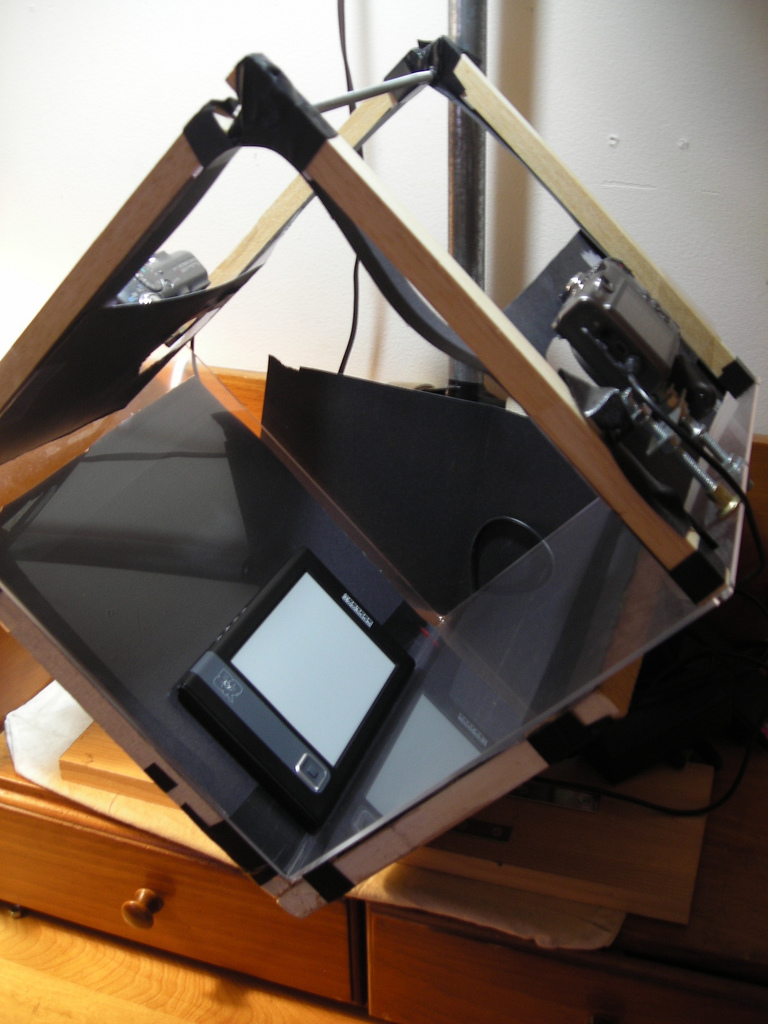
\includegraphics[width=7.1cm]{flickr_e-book-ripper}
   \caption{e-book ripper (Copied from bkrpr.org (2009) \cite{flickr:e-book_ripper}).}
   \label{fig:def:e-book_ripper}
\end{figure}
because the best e-book DRM will suffer from the analog hole. In other words, the protection ends once displayed on screen. So anyone with a digital camera and an Optical Character Recognition (OCR) software can get an almost perfect DRM-free copy in few minutes. For example, in figure \ref{fig:def:e-book_ripper}, a book ripper designed to digitalize physical book\footnote{Where the book is placed in the middle and when turning every pages, take a picture of the odd page with the left camera (the right one for the even page). When the end of the book is reach, the pictures are treated with an OCR software that will produce the e-book.} is used to free up a DRM protected e-book from a reader device. 

Another fear for the user is if the vendor goes bankrupt or if the DRM provider stops to maintain the system. This happen with Microsoft\label{def:opp_ms} announcing that they will not support any more the .lit file format: \textquotedblleft Microsoft is discontinuing Microsoft Reader effective August 30, 2012, which includes download access of the Microsoft Reader application from the Microsoft Reader website\textquotedblright ~\cite{microsoft:reader}; so the users may loose the access to their files when their devices will die. 

Since the DRM can also be location aware\footnote{the patents exist (e.g. \url{http://appft1.uspto.gov/netacgi/nph-Parser?Sect1=PTO1&Sect2=HITOFF&d=PG01&p=1&u=/netahtml/PTO/srchnum.html&r=1&f=G&l=50&s1=20060059096.PGNR.})}, it can be problematic for the user who travel or move abroad. This can also impede a user to buy a book from an other country if for example, the book is not available in his area (Apple iBooks store is not accessible in every countries). This looks again like a way to control the business. 

Illegal offers exist for e-books; but it is minority. Based on a French survey, it count only for 5\% through file sharing websites, 4\% with peer to peer (P2P) and 1\% in streaming\footnote{except for streaming, the study do not specify if the download was legal or not (e.g. an e-book under a creative common license (or in the public domain) can be legally downloaded via P2P).}; compare to legal offer with 41\% through the big operator (Amazon, Apple Store, Google books, etc.) and 28\% on specialized web-stores (Fnac, VirginMedia, Cultura, etc.), etc. \cite[p. 9]{OpinionWay:baro_v2}. The same survey also reports that 17\% of the readers had at least once acquired an e-book illegally. The reasons in doing so was for 69\% that the legal offer was too expensive, for 40\% that the legal offer did not exist and for 14\% that there were having problems with DRM \cite[p. 13]{OpinionWay:baro_v2}. So, to reduce the download of e-books, the publishers/vendor could concentrate on attractive and/or transparent\footnote{e.g. in Finland the Value Added Tax (VAT) is 23\% for e-book while it has a reduced rate of 9\% for paper book (\url{https://www.vm.fi/vm/en/10_taxation/04_value_added_tax/index.jsp}).} price, have richer collections available and abandon DRM. 

Going DRM-free can have a positive impact on the readers and be used as a marketing argument. In facts, Bragelonne, a French publisher, followed that path in the end of 2010. Six month later, they reported that this strategy made them among the leaders in e-books selling in their genre. The journalist use that success-story as an extra example to show that the \textquotedblleft DRM is a barrier to business\textquotedblright ~\cite{numerama:drm}. More generally, being DRM-free does not prevent to do business. 

Watermark and Social DRM also raise some privacy concerns, like the risk of having private data (such as the reader full name, email, the credit card number, etc.) visible to everyone. They can also lead to an unfair punishment if for example, someone loose his reading device and his files goes illegally shared, he risks to be punished for crime he did not committed. And this can also affect people who have a poor knowledge of technology, who can by mistake make their files available to the public.

With DRM, Watermark and Social DRM, the reader must provide private information in order to purchase an e-book. He don't has the possibility to buy it anonymously as he could do with physical book by paying cache in a bookshop. This could lead to self-censorship where the user would refrain himself from buying a controversial e-book with the risk of restricting his freedom of opinion.

%http://edri.org/campaigns/copyright
%http://www.edri.org/docs/edri_copyright_consultation.pdf
%http://ec.europa.eu/internal_market/copyright/studies/studies_en.htm

\section{DRM Alternative}

The file sharing on internet (authorized or not) is a reality and the DRM does not stop nor prevent it. So, an alternative to the technical measure is to have no DRM. Among the advocates of such approach, let mention Stallman \cite{gnu:freedom_or_copyright} with his essay Freedom\textemdash or Copyright? and Aigrain \cite{aigrain:sharing} with his book Sharing. Both also promote the legalization of non-market file sharing. The non-market file sharing is done between users without commercial counterpart and without using a commercial third party service.

Stallman \cite{gnu:freedom_or_copyright} and Aigrain \cite[section 3.2]{aigrain:sharing} say that non-market sharing is useful for culture by providing a better access to it, making it more divers and also by making available out of print and orphan works. It can also help in promoting unknown authors, when publishers put focus on possible best-selling tittle (from which they hope to get more revenues), the readers will more likely share works that they enjoyed or think that are of interest. 

They also say that the authors can still get fair revenues by selling DRM-free e-books giving example of Stephen King \cite{gnu:freedom_or_copyright} and even e-books release under the Creative Commons licenses in synergy with paper books such as Cory Doctorow or John Sundman \cite[section 7.4]{aigrain:sharing}. In scientific/technical publishing, this is already a reality with publishers like Springer who provide e-books with no DRM to guarantee \textquotedblleft Perpetual access \& ownership\textquotedblright ~\cite{springer:ebooks} or O'Reilly who adds services to attract customers such as \textquotedblleft lifetime access\textquotedblright , provide the files in multiple formats so the user can read them in any device and \textquotedblleft free updates to reflect published changes and corrections\textquotedblright ~\cite{oreilly:ebook}. 

In fiction and others genre, some vendors, for example, Weightless Books\footnote{\url{http://weightlessbooks.com/about/}} sell all their e-books DRM-free. In publishing the Tor/Forge announced that they will release their full catalogue without DRM by July 2012 \cite{tor:drm-free} and that discussion went with their parent company Macmillan \cite{antipope:more_drm}. One of the older DRM-free publisher is Baen Books\footnote{\url{http://www.baenebooks.com/t-DRM.aspx}} who was in 2007 stating:
\begin{quote}
We don't treat our customers like criminals, and they don't act like them. We've found that if you treat your readers with respect, they become repeat customers, as the success of our decade-old Webscription program can attest. \cite{baen:subterranean}
\end{quote}

An alternative way of selling e-book was experimented by Humble Bundle\footnote{\url{http://www.humblebundle.com}}. They offered a bundle of thirteen DRM-free e-books during two weeks with the \textquoteleft Pay What You Want\textquoteright ~pricing system and a possibility to set a percent that will go to charity. The result was over 84 thousand purchases of the bundle generating 1,2 million \textdollar ~\cite[Humble eBook Bundle]{humble:eBook}. This was seen successful enough to give birth to the story bundle\footnote{\url{http://storybundle.com/}} based on the same principle. 

Stallman \cite{gnu:freedom_or_copyright} and Aigrain \cite[section 5.2, chapter 6 and 7]{aigrain:sharing} also propose a new source of income for the authors to remove their fear to publish their works DRM-free in digital form. The idea is to collect a flat-rate tax based on internet subscribers that would be redistributed to authors and how that would be distributed. Aigrain goes further by proposing that the collected money should also fund future cultural project and a part to serve for archiving. 

Aigrain ~\cite[chapter 6]{aigrain:sharing} also provides more idea about the rights to share; the sharing of cultural artefacts would be possible only after they have first been made available to the public in digital form. For example, scanning a paper book and sharing it will still be copyright infringement; except if the author has explicitly permitted it. \textquotedblleft This saves an essential element of media chronology: the possibility [for the author] to schedule the public performance, analogic distribution and digital distribution at different times\textquotedblright . In addition to the sharing, he proposes the remix right to create modified works. He also insists on the facts that the users must respect the attribution of the authors for their works and can’t remove nor modify the meta-data identifying a file. With Stallman \cite{gnu:freedom_or_copyright}, they insist on the non-market sharing part. For example, websites that want to sell copies, give direct access to a library of files through subscription system or by using ads will still need to negotiate commercial licenses with the authors. 

At the political level, the \textquoteleft free culture\textquoteright ~ is a motto of the pirate parties\footnote{\url{http://piraattipuolue.fi/english }}. The idea is also supported by the European Green Party \cite{green:digital_right}. The subject is discussed at various stages in some governments such as France, Belgium, Germany, Brazil and Switzerland where a postulate \textquotedblleft toward a fair copyright compatible with internet user freedom\textquotedblright \footnote{my translation} \cite{parlement:12.3326} has been proposed and has been accepted by the government who has formed a working group\footnote{\url{http://www.ejpd.admin.ch/content/ejpd/fr/home/dokumentation/mi/2012/2012-08-09.html} (in French (also available in German and Italian))} that will provide the results at the end of 2013. 

Stallman \cite{gnu:freedom_or_copyright} concludes by advising that before this \textquotedblleft information utopia\textquotedblright ~battle is won, the users should not buy DRM products \textendash except if there is a way to break it\textendash ~to avoid the establishment of a \textquotedblleft pay-per-view world\textquotedblright ~ imposed by publishers. 

\chapter{Results}

The main products of this thesis are the participation for the Next Media project in different forms. One is the deliverable (number 1.3.1.4) with the title \textquotedblleft Protection mechanisms for
electronic books\textquotedblright . It is composed of almost the same text and content as the chapters \ref{intro}, \ref{protec}, \ref{exist}, \ref{free} and \ref{conc} as of this work. It was returned to the consortium in February 2013. A copy of this document can be found in github\footnote{\url{https://github.com/patrick-ausderau/thesis}}.

Another participation to the Next Media project consisted of a presentation to the Finnish National library and the company Ellibs representatives in April 2012. The presentation and discussion concentrated on the topics of how could Finnish libraries lend e-books as they do with paper books and also about the archiving e-books. An other presentation for the Finnish Book Publishers Association development group in October 2012 concentrated in presenting the different alternatives for protecting e-books.

For the eReading work-package of the Next Media project, there are two presentations in seminars, one in June 2012 and the next one in December 2012. Another seminar participation is the Next Media Result Seminar in February 2013, with a short, fifteen minutes presentation. The slide show of this presentation is available in the Next Media website\footnote{\url{http://www.nextmedia.fi/779350088/en/read/Next_Media_Result_Seminar_6.2.2013}} and the video recording available on the Vimeo platform\footnote{\url{http://vimeo.com/59498270}}. A last presentation is a 45 minutes conference for the Finnish Book Publishers Association and two authors unions members in February 2012. The slide show of all the presentation are published in github\footnote{\url{https://github.com/patrick-ausderau/thesis}}.

The last task for the Next Media project is the participation to the reflection group about e-book protection initiated by the Finnish Book Publishers Association. The outcome is the DRM recommendation send to the Finnish publishers in June 2013. The main result being majors Finnish publishers who abandon DRM in favour of the watermark and Social DRM lighter protection system \footnote{\url{https://www.sttinfo.fi/release?releaseId=8700912}}. The Web crawler text is accompanying the DRM recommendation. It is presented in the annex \ref{app:crawl} or as a stand alone text in github\footnote{\url{https://github.com/patrick-ausderau/thesis}}

The application produced for this thesis demonstrates that the upcoming W3C Web Cryptography API can be used to encrypt data. It also shows some of the limitation of DRM systems such as the difficulty to hide private key. It also outline the risks in using the current implementation of the Web Cryptography API for serious cryptographic operations.


\chapter{Discussion}\label{discuss}

During this research work, I studied the existing and upcoming protection techniques on e-book, namely: Digital Right Management (DRM), Watermark, Social DRM and Lightweight Content Protection (LCP) and tried to implement a protection system with the Web Cryptography API. What I found is that it does not exist possible improvement of the DRM techniques because of the paradigm problem of trying to impose the physical world to the electronic world which are fundamentally different.

However, a technical solution that could guarantee a fair revenue to the author of a e-book while not restricting the user freedom to share copy of it, could be to implement a script that would present to the reader a donate button. With such button, if the reader likes the e-book, he could very easily offers to the author a small sum of money as a reward for his work. A similar system already exist on the internet with for example Flattr\footnote{\url{https://flattr.com/}}.

At the non technical level, there is also important lewis that can be used to fight copyright infringements. At the market level, it is important that the publishers offer a rich collection of titles in electronic form, makes it easily available, propose attractive prices and ideally do not impose DRM restriction. With that approach, the user would be less tempted to search for the illegal alternatives. Another approach that would be interesting to study could be to test Crowdfunding where the author writes and publishes his new book only if he gets its funding beforehand.

Another important lewis is to continuously educate people about the copyright. With Crowdfunding or a donate option, this work could be made easy as \textquotedblleft did you offer 1\euro to your favourite author this month?\textquotedblright ~\cite{gnu:freedom_or_copyright}. Finally, the other proposition is to collect flat-rate tax that would be distributed to the authors. Such proposition requires a work at the political and legal level in order to adapt the copyright laws to the reality of the internet.

While this research work was limited to the protection of electronic book, many of these proposition could be extended to the arts and sciences in general. This problem and the proposed solution already apply to the music and cinema and with the advance of technology such as 3D printer, this could also reach other domains such as sculpture and carving. There is research on holographic screen, so maybe one day, we will be able to have live arts such as dancing and theatre in our living room as well.

\chapter{Conclusions}\label{conc}


The research conducted shows that among the technical options to protect e-book from illegal uses, none is perfect. Trying to impose the rules of the physical world to the electronic one is not suitable. 

For the e-book, the \textquoteleft hard DRM\textquoteright is not an appropriate solution as it does not prevent nor stop the illegal file sharing, it restricts the freedom of legitimate reader (while cracker get it fully), adds extra costs in term of price and infrastructure for the publisher/vendor and tends to fragment the market (or creates monopoly). However, in some cases, such as company confidential documents, where the reader and provider agree on the need for protection, the DRM may be a good solution. 

Concerning the Lightweight Content Protection (LCP), it remains interesting on following the IDPF work. Even if the LCP still has unclear costs, it could be an alternative to \textquoteleft hard DRM\textquoteright for vendor or library when the publisher imposes technical protection. If it would be implemented, it could also reduce some of the drawbacks with better interoperability, no spying and a real ownership for the reader. But, as with the \textquoteleft hard DRM\textquoteleft , it could be cracked or the users may fight against it. 

The Social DRM and watermark combination might be the less problematic solution. It can be better accepted by the users, offers some level of protection and help deter on copyright infringement. However, the reader may reject it because of privacy concern.

For these reasons, being DRM-free would be the better option. It might show that the authors trust and respect their readers. Copyright and licenses, such as the Creative Commons, do provide protection and being DRM-free does not prevent to do business. It is also relevant to continue the work at the educational, legal and market levels. 


%=================== BIBLIOGRAPHY =================
\bibliographystyle{vancouver}
%\bibliographystyle{plain}
%line space
%\singlespacing
\begin{flushleft}
\begin{singlespacing}
\bibliography{biblio}
\end{singlespacing}
\end{flushleft}

%\bibitem{e-book_use} Umut Al; Irem Soydal; Yasar Tonta. \textit{Analysis of E-book Use: The Case of Ebrary}. In: 14th International Conference on Electronic Publishing, Helsinki. 2010. Available at \url{http://eprints.rclis.org/bitstream/10760/14696/1/tonta-al-soydal-ELPUB2010-Analysis-of-e-book-use.pdf} (12 January 2012).

%\end{thebibliography}

%for conting the pages
\label{LastPage}~
\clearpage

%=================== APPENDICES =================
\appendix
%\linespread{1.5}
%no page number for appendix in table of content
\addtocontents{toc}{\cftpagenumbersoff{chapter}}
%appendix sections and subsections not in table of content
\settocdepth{chapter}
%add Appendices in the table of content
\addappheadtotoc
%have Appendix 1 (instead of Appendix A)
\renewcommand{\thechapter}{\arabic{chapter}} 

%special counter for appendix
\setcounter{page}{1}
\newtotcounter{appage1}
%overwrite the header
\makeevenhead{plain}{}{}{Appendix \thechapter \\ \thepage (\stepcounter{appage1}\total{appage1})}
\makeoddhead{plain}{}{}{Appendix \thechapter \\ \thepage (\stepcounter{appage1}\total{appage1})}


\chapter{Web Crawler}\label{app:crawl}

Pant et al. \cite{inweb:crawling} define \textbf{Web Crawlers} as programs that exploit the graph structure of the Web to
move from page to page. Crawlers are also known as spiders, robots or simply bots, and in their infancy were also named wanderers, fish or worms. In 1993, the first web crawler, the World Wide Web Wanderer\footnote{\url{http://www.mit.edu/people/mkgray/net/background.html}}, was used to compile statistics about the growth of the web \cite{naj:crawl}. They quickly became a central component of search engines to collect web pages that are to be indexed (for example the googlebot\footnote{\url{http://support.google.com/webmasters/bin/answer.py?hl=en&answer=182072}}). Crawlers are used for many other applications such as archiving the web (e.g. Heritrix\footnote{\url{https://webarchive.jira.com/wiki/display/Heritrix/Heritrix}} crawler) or specialized data mining, for example for price comparison services (e.g. the ShopWiki\footnote{\url{http://www.shopwiki.com/w/Help:Bot}} crawler) or searching for copyright violation (e.g. the Digimarc Guardian\footnote{\url{http://www.attributor.com/solutions/solutions.php?X=1.1}} or the Belgian Librius SINBAD\footnote{\url{http://www.librius.com/over-librius/wat-doet-librius/Librius-SINBAD/}} crawlers) and more (e.g. spambot (used to collect email addresses and send unsolicited messages), etc.). 

The operations of web crawlers, as described by Manning et al. \cite[pp. 405-420]{man:info_ret}, are as follow:
\vspace{-17pt}\begin{enumerate}
\setlength{\itemsep}{0cm}%
\setlength{\parskip}{0cm}%
\item The crawler starts with one or more web page addresses constituting the \textit{seed set}, picks one URL\footnote{Uniform Resource Locator} from the set and download that web page.
\item The fetched page is then parsed with two objectives:
	%\vspace{-5pt}
	\begin{enumerate}
	\setlength{\itemsep}{0cm}%
	\setlength{\parskip}{0cm}%
	\item Extract the text, images, etc. for the data mining process, or in the case of a search engine to fed the indexer.
	\item Extract the links to other pages, files, etc. that are added to a \textit{URL frontier}, corresponding to the resources that have yet to be fetched by the crawler. Initially, the URL frontier contains the seed set.
	\end{enumerate}%\vspace{-4pt}
\item Once the resource has been fetched and parsed, its URL is either removed from the URL frontier or time stamped for a later visit.
\end{enumerate}
\vspace{-9pt}
Manning et al. \cite[pp. 405-420]{man:info_ret} also list the features web crawler must or should provide. Ideally, a crawler must be \textbf{robust} to avoid spider trap, which are server generating web pages making the crawler downloading million of pages from the same domain and be \textbf{polite}. The politeness is both implicit, for example the crawler will wait some time before downloading a page from the same domain to avoid server overloading and bandwidth consumption and explicit by following the Robots Exclusion Protocol define in the robot.txt\footnote{\url{http://www.robotstxt.org/}} which set what resources a crawler can or not visit and fetch. Malware and spam robots are know to not follow these rules and some commercial crawler such as the Attributor (now Digimarc Guardian) do not respect the exclusion neither, even if understandably necessary, webmasters may block it more aggressively\footnote{\url{http://incredibill.blogspot.fi/2007/11/attributor-post-mortem-copyright.html}}. The features crawler should have concern efficiency, quality, freshness, scalability, extensibility, etc.


%============== USE CASES ==========================
\clearpage
\setcounter{page}{1}
\newtotcounter{appage2}
%overwrite the header
\makeevenhead{plain}{}{}{Appendix \thechapter \\ \thepage (\stepcounter{appage2}\total{appage2})}
\makeoddhead{plain}{}{}{Appendix \thechapter \\ \thepage (\stepcounter{appage2}\total{appage2})}

\chapter{Use Cases}\label{ebook:uc}

In this chapter will be presented an exhaustive list of actions that can be perform with e-books in form of use cases. %The actions are grouped into logical sets 
First comes the definition of the user roles. These actors are the users who interact with the e-books:
\begin{description}[leftmargin=2.3cm, style=sameline] %\itemsep1pt%leftmargin=2.3cm, style=sameline
\item[Author] A person or a group of person who create (write the text, draw illustration, etc.) a book.
\item[Individual] Refers to a single person who read an e-book.
\item[Teacher] Is a person whose work is to bring knowledge to others (usually students).
\item[Researcher] A person or a group of person running studies on a specific subject in order to reach a new understanding or discovering new information~\cite{cambridge:dictionary:researcher}.
\item[Publisher] A company or a person who publish books and e-books and promote them.
\item[Seller] A person or a company who sell or rent e-books.
\item[Library] Is an institution who make available to the public by lending cultural, educational and research material, such as books, magazines, CDs, films, etc. A library is also responsible for maintaining such material collection and may also serve for archiving it for future generations~\cite{thefreedictionary:library}.
\end{description}


%\vspace*{11pt}
\section{Detailed Use Cases: Read, Buy, Borrow, Lend, Rent, Offer, Resell, Annotate an E-book}\label{uc:read_buy}


\textbf{Use case: Read an e-book}\label{uc:read}

Actors: Individual, Teacher, Researcher.

%\vpageref{uc:buy}
Prerequisite: The user got an e-book either by buying it (cf. \vref{uc:buy}) or borrowing it (cf. \vref{uc:borrow}). He has an appropriate device (computer, tablet, etc.) and there is an application installed on it able to open and display the e-book.

Story: The user has open the reading application on his device. From the application, he clicks the open menu, browses where the e-book file is located and selects it. The application opens the e-book at its first page. At this stage, the user can start reading.\\
Usually the reading application will also provide to the reader some navigation facilities like moving forward/backward to the next/previews page, going to a specific page, chapter, bookmark (see \vref{uc:annotate}), etc. Such application can also provide zooming (make the text smaller/bigger) functionalities.

\begin{figure}[h]
   \fbox{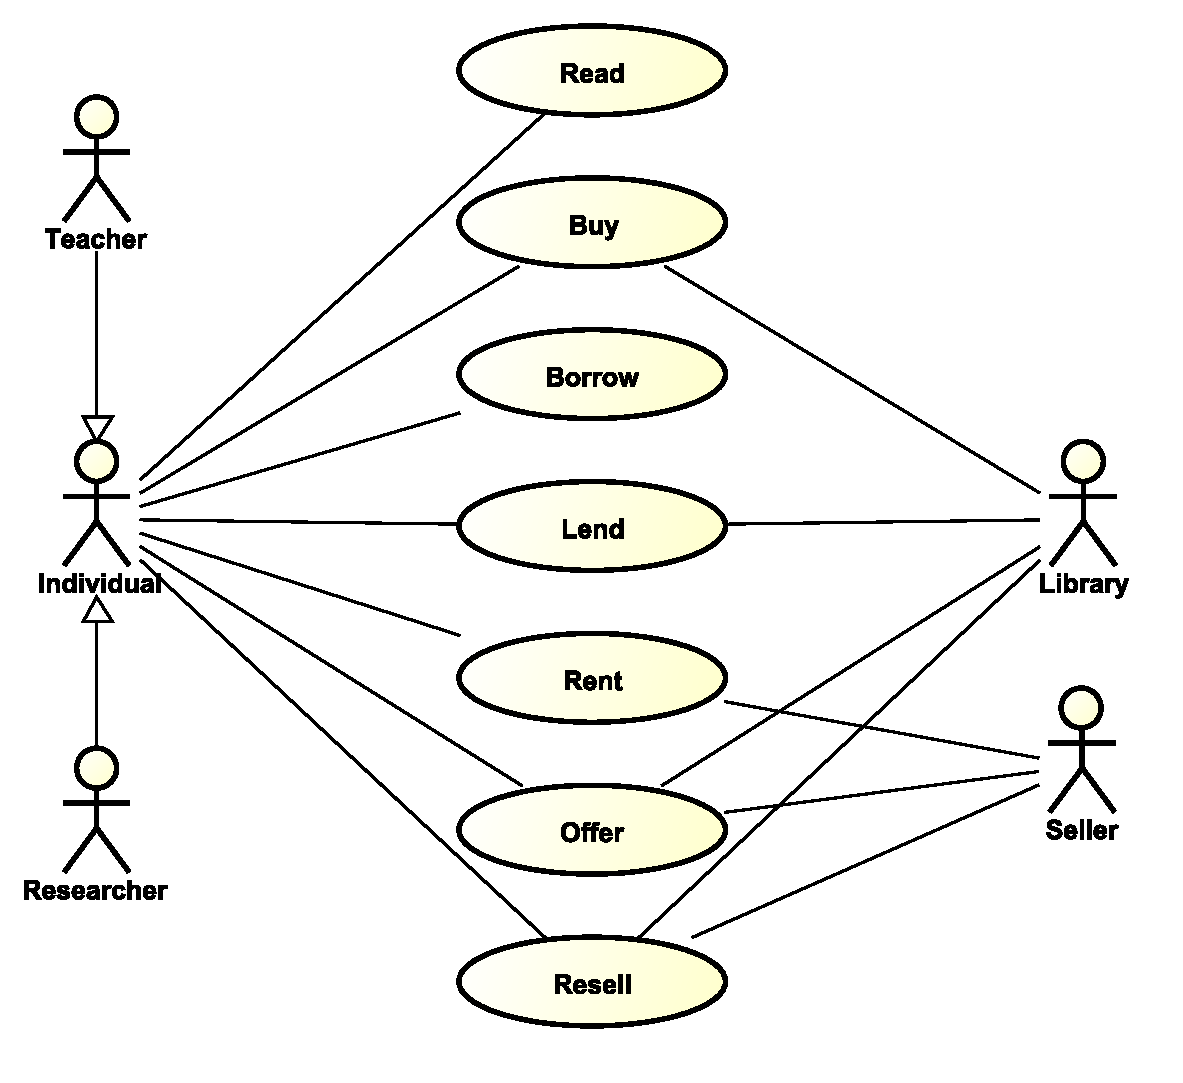
\includegraphics[width=14.9cm]{uc_read_buy}}
   \caption{Use case diagram for section \ref{uc:read_buy}: Read, Buy, Borrow, Lend, Rent, Offer, Resell an e-book.}
   \label{fig:uc:read_buy}
\end{figure}

\textbf{Use case: Buy an e-book}\label{uc:buy}

Actors: Individual, Teacher, Researcher, Library.

Prerequisite: The user has an appropriate device with an internet connection (in here the assumption is that the buying transaction will be done on the internet through an on-line book store) and a web browser. He also disposes of a payment method (through credit card, paypal, etc.).

Story: The user uses his web browser to navigate to the on-line book store. There, he will browse the list of available e-books or use a search facility. Once the user finds the e-book he wants, he orders it (usually by adding it into a shopping cart). By confirming the order, he will be requested for payment (e.g. with credit card). Once the payment is confirmed he will get his e-book through download. The user now owns the e-book and has it as a file on his device.\\
An alternative would be that the e-book goes on the cloud (cf. \ref{uc:cloud}), in that case the e-book file is not downloaded on the user device but is stored on-line.
%\vref

\textbf{Use case: Borrow an e-book}\label{uc:borrow}

Actors: Individual, Teacher, Researcher.

Prerequisite: A lender makes an e-book available (cf. \vref{uc:lend}) to the user on-line through a website, by sending it by email, by sharing it with a social network website or by sharing it with a physical storage medium such as a memory card, USB flash drive, etc. The user has an appropriate device (computer, tablet, etc.) and there is an application installed on it able to open and display the e-book.

Story: The user navigates where the e-book is (e.g. the library website, the sharing place of another user, etc.). He specifies the borrowing period (usually a few hours to a couple of weeks) if not predefine by the lender. The user then retrieves (e.g. by downloading) the e-book file. He now has the read access for the borrowing period. At the same time, the lender looses his read access for that same period.\\
There should be also option for the user so he can return the e-book before the end of the borrowing period and/or a symmetrical option where the lender can request the e-book back.

\sout{Alternative story for library: A library owns 5 copies of an e-book and all five copies are borrowed. A user does not want to wait that one of the e-books comes back. The library will charge a fee from the user and use that money to get a temporary extra copy from the publisher and lends that extra copy to the borrower. This is not to be confused with the renting (cf. \vref{uc:rent}) use case; in here the library does not make any benefit, the fee goes integrally to the publisher for getting the temporary extra copy of the e-book.} 2012-01-30 Olli meeting about library DRM => concerning libraries,
for the customers borrowing have to be free of charge!


\textbf{Use case: Lend an e-book}\label{uc:lend}

Actors: Library, Individual, Teacher, Researcher.

Prerequisite: The user owns an e-book. He has a device, where the e-book is stored, with an internet connection or a connector for a removable storage medium. The borrower will have to have the symmetrical device facilities. The lender has an application installed on his device that help him to modify the e-book access rights.

Story: The user changes the rights of his e-book to the lend state. He specifies the lending period (from few hours to couple of weeks) or alternatively provides a lending range (so the borrower will decide how long he will borrow it). The user puts his e-book on-line (through a website, a social network website) or sends it by email or puts it on a physical storage medium. Once the borrower gets the e-book file, he instantly gets the read access to it and at the same time, the lender looses his read access and his right to lend it (to avoid concurrent lending or  renting (cf. \vref{uc:rent}) of the same e-book) for that same lending period.\\
There can be an option where the lender can request the e-book back before the end of the lending period and/or an option for the borrower to return it earlier.

\textbf{Use case: Rent an e-book}\label{uc:rent}

Actors: Seller, Individual, Teacher, Researcher.

Prerequisite: The owner of the e-book has a device, where the e-book is stored, with an internet connection or a connector for a removable storage medium. The renter will have to have the symmetrical device facilities. The owner has an application installed on his device that help him to modify the e-book access rights. 

Story: The owner changes the rights of his e-book to the rent state. He specifies the renting period (typically from few hours to couple of weeks). Once the renter pays the fee, he gets (by downloading or through removable storage medium) the e-book on his device. He has now the read access to the e-book for the renting period. At the same time, the owner looses his right to read and rent the e-book (to avoid concurrent renting or lending (cf. \vref{uc:lend})) for that same period. \textbf{TO CHECK: DOES THE OWNER HAS TO PAY A SPECIAL TAX TO PUBLISHER/AUTHOR OF THE E-BOOK?}

Alternative story: The seller (owner) can rent as many copies of the e-book he wants. In that case he will pay to the publisher (or the author) an extra fee per rented copies. The idea here is to propose a business approach similar to VOD (Video On Demand).

\textbf{Use case: Offer an e-book}\label{uc:offer}

Actors: Individual, Teacher, Researcher, Seller, Library.

Prerequisite: The owner of the e-book has a device, where the e-book is stored, with an internet connection or a connector for a removable storage medium. The receiver will have to have the symmetrical device facilities. The owner has an application installed on his device that help him to modify the e-book access rights.

Story: The user modifies the ownership of the e-book to be the receiver. He then offers the e-book to that person. He looses all the rights on the e-book. The receiver now owns the e-book and has the full rights (read, lend, etc.) on it.\\
For a library, if they want to reduce storage (like save server disk space), they can offer e-books that were only rarely borrowed.\\
For a seller, he can offer e-book for good customer or make special offers like buy ten e-books and pay for nine.

\textbf{Use case: Resell an e-book}\label{uc:resell}

Actors: Individual, Teacher, Researcher, Seller, Library.

Prerequisite: The owner of the e-book has a device, where the e-book is stored, with an internet connection or a connector for a removable storage medium. The buyer will have to have the symmetrical device facilities. The owner has an application installed on his device that help him to modify the e-book access rights.

Story: Once the user gets the money payment from the buyer, he modifies the ownership of the e-book. He then transmit (through internet, email or with a removable storage medium) the e-book to the buyer. The buyer now owns the e-book and has the full rights on it. At the same time, the ancient owner looses them.\\
Library sometimes resell books that were rarely read (or broken); so something similar may append with e-books. That allow them to free some space (in this case, disk space).\\
For a seller, we can image a system similar to a second hand shop where they buy e-books from individuals and resell them.


\textbf{Use case: Annotate an e-book}\label{uc:annotate}

As define in the W3C Incubator Use Case Social Annotation~\cite{w3c:uc_annotation}, is consider as an annotation: a bookmark, line mark that the reader can use to quickly navigate to a specific part of the e-book (as example remember where he stop reading to restart reading from there); a comment about a sentence, paragraph, chapter, the all e-book; a summary or a description of the e-book or part of it; etc.

Actors: Researcher, Teacher, Individual.

Prerequisite: The owner of the e-book has a device, where the e-book is stored, with a reading application that help him to add bookmark. He may also have another application that allow him to write text (a notepad), record voice, etc.

Story: The user reads or browses the e-book to a specific place (page, line, chapter, etc.) and mark it. By saving this mark, he already has a bookmark. He then write his comment in a text editor or record his voice comment. He optionally add a title or a description of his comment. By aggregating the comment with the bookmark, he has created an annotation.

\section{List of Other Use Cases}

The use cases were the very start point of this work. The goal of it was to get an as complete as possible overview of all the possible actions that can be done with an e-book in its larger definition (the file, application and/or device). While relevant, they did not feet well in the thesis itself and went into this annex. When that decision was took, the formal writing of the use cases was stopped. The table \ref{uc:table} presents the others cases that are not described in the section \ref{uc:read_buy}. The description of the use cases is using keywords only and could be harder to read.

\begin{table}[h]
  \centering
  \caption{Short version of use cases}
  \begin{tabularx}{.99\textwidth}{|p{.25\textwidth}|X|}
    \hline
    \multicolumn{1}{|c|}{\textbf{Use Case}} & \multicolumn{1}{c|}{\textbf{Description}} \\
    \hline
    Share annotations of an e-book & Prerequisite: The user has created an annotation (cf. \vref{uc:annotate}). -internet connection - personal website, social network website, etc.

Stories: shares his annotations - accesses and uses others annotations \\
    \hline
    Copy an e-book & backup, archive, transfer on multiple devices (e.g. using a USB stick) \\
    \hline
    Copy (part of) the content of an e-book & for a quotation, for a review, etc. \\
    \hline
    Offer a copy of an e-book & Like offer but the original owner keep a copy of the book.
    
    Note: Require author consent \cite[Article 4.1]{eur-lex:2001/29/EC} or not e.g. if under any of the creative commons licenses (even the NC).\\
    \hline
    Sell a copy of an e-book & Same as offer; but with money transaction. It almost become a parallel distribution.
    
    Note: Require author consent \cite[Article 4.1]{eur-lex:2001/29/EC} or not e.g. if under some of the creative commons licenses (all that are not NC).\\
    \hline
    Print an e-book & Does that become a physical book? \\
    \hline
    Offer printed copy of (part of) an e-book & E.g. for teacher, as teaching material \\
    \hline
    Sell printed copy of an e-book & To check if illegal? \\
    \hline
    Convert an e-book to another format & E.g. some device/application require a specific format (can not read the others) \\
    \hline
    Read on multiple devices & E.g. user start to read in the train on mobile phone and continue home on the computer. Requires to have copies on multiple devices. Synchronization would be nice to have (continue to read on the next device where stopped on the previous). \\
    \hline
    Read on multiple devices concurrently & E.g. Wife on the mobile phone and husband on the computer. Requires to have copies. \\
    \hline
    publisher / vendor cases & Sell
    
    Return to shop for resale (after reading, keep a copy)
    
     DRM-free after entering the public domain
     
     Access after publisher/seller bankrupt
     
     Track/trace
     
     preview and other promotion mechanism\\
    \hline
    Archive & As a backup, keep a copy on another machine/disk in case of crash or as a pure archiving for the future generation. 
    
    Similar to the copy case. \\
    \hline
        \end{tabularx}
  \label{uc:table}
\end{table}

%very hugly way of cutting the table... but the longtabu was compressing it into one page instead of cutting in into many :(
    \begin{tabularx}{.99\textwidth}{|p{.25\textwidth}|X|}
    \hline
    \multicolumn{1}{|c|}{\textbf{Use Case}} & \multicolumn{1}{c|}{\textbf{Description}} \\
    \hline
    Store a copy of an e-book on the cloud\label{uc:cloud} & keep a copy on a distant server that can easily be accessed by different devices over the internet.
    
    Similar to copy and archive cases. \\
    \hline
    anonymously buy/own/borrow an e-book & E.g. if you are interested in religion and science, you do not want to be blocked at the border because you have read the Koran and chemistry books.  \\
    \hline
    Use as teaching/research material & More because it is one of the exception \cite[Article 5.3(a)]{eur-lex:2001/29/EC}. 
    
    Requires the copy content, print cases and more. \\
    \hline
    Share library & Offer a collection of e-books. Or share the list of e-books that other users could borrow. \\
    \hline
    E-book swapping & similar to the book swapping, once read, offer the e-book to a friend in exchange of one of his e-book. \\
    \hline
    BookCrossing & Require a physical book. BookCrossing a reading device with e-books on it? \\
    \hline
  \end{tabularx}

%============== SOFTWARE ==========================
\clearpage
\setcounter{page}{1}
\newtotcounter{appage3}
%overwrite the header
\makeevenhead{plain}{}{}{Appendix \thechapter \\ \thepage (\stepcounter{appage3}\total{appage3})}
\makeoddhead{plain}{}{}{Appendix \thechapter \\ \thepage (\stepcounter{appage3}\total{appage3})}

\chapter{Source Code}\label{source:code}

The \url{genkey_and_export.html} HTML file in listing \ref{source:html} is the starting point of the application where the user is presented the action of generating the public and private key pair, export the public key by calling the \url{keydecrypt.js} and shares it with the distant server by sending it to the \url{encrypt.php}.

\lstinputlisting[language=HTML,caption={Generates keys and exports - HTML file},label=source:html]{genkey_and_export.html}

The \url{keydecrypt.js} JavaScript file in listing \ref{source:js} is responsible for the operation on the client side. It generates the public and private keys pair, exports the public key and decrypts the content of files with the private key.

\lstinputlisting[language=JavaScript,caption={Generates keys, exports public key and decrypts - JavaScript file},label=source:js]{keydecrypt.js}

The \url{encrypt.php} PHP file in listing \ref{source:php} handles the server side operations. It imports the user public key and uses it to encrypt a EPUB file content that is sent back to the user for decryption and rendering.

\lstinputlisting[language=PHP,caption={Imports public key, encrypts content - PHP file},label=source:php]{encrypt.php}

%============== SEMINAR ==========================
%\clearpage
%\setcounter{page}{1}
%\newtotcounter{appage4}
%overwrite the header
%\makeevenhead{plain}{}{}{Appendix \thechapter \\ \thepage (\stepcounter{appage4}\total{appage4})}
%\makeoddhead{plain}{}{}{Appendix \thechapter \\ \thepage (\stepcounter{appage4}\total{appage4})}

%\chapter{Semiar Sildes Sample}\label{semiar}

%This is the slides produced for the presentation for the Finnish Book Publishers Association in February 2012.

%
\includegraphics[width=13cm]{e-book_protection_seminar}

\end{document}